% =============================================================================
%  SPECTRA_final.tex  :  Single compilable paper file
%  Spectral-Probabilistic Ensemble Clustering for Transaction Recognition
%  and Authentication
%  Target : IEEE Transactions on Information Forensics & Security
%  Author : Sagar Korde
%
%  Compile with:
%    pdflatex SPECTRA_final.tex
%    bibtex   SPECTRA_final
%    pdflatex SPECTRA_final.tex
%    pdflatex SPECTRA_final.tex
% =============================================================================

\documentclass[journal]{IEEEtran}

% ── Core packages ─────────────────────────────────────────────────────────────
\usepackage{amsmath,amssymb,amsthm}
\usepackage{booktabs}
\usepackage{graphicx}
\usepackage{xcolor}
\usepackage[hidelinks]{hyperref}
\usepackage{url}
\usepackage[group-separator={,}]{siunitx}
\usepackage{enumitem}
\usepackage{algorithm}
\usepackage{algpseudocode}
\usepackage{multirow}
\usepackage{array}
\usepackage{microtype}
\usepackage{bm}
\usepackage{mdframed}
\usepackage{rotating}
\usepackage{tabularx}
\usepackage{threeparttable}
\usepackage{placeins}
\usepackage{tikz}
\usepackage{pgfplots}
\pgfplotsset{compat=1.18}
\usetikzlibrary{arrows.meta, positioning, shapes.geometric, fit, backgrounds,
                decorations.pathreplacing, calc}

% ── Theorem environments ──────────────────────────────────────────────────────
\newtheorem{definition}{Definition}
\newtheorem{problem}{Problem}[section]
\newtheorem{theorem}{Theorem}
\newtheorem{remark}{Remark}

% ── Short-hand macros ─────────────────────────────────────────────────────────
\newcommand{\spectra}{\textsc{SPECTRA}}
\newcommand{\R}{\mathbb{R}}
\newcommand{\calG}{\mathcal{G}}
\newcommand{\calV}{\mathcal{V}}
\newcommand{\calE}{\mathcal{E}}
\newcommand{\bx}{\mathbf{x}}
\newcommand{\bz}{\mathbf{z}}
\newcommand{\bh}{\mathbf{h}}
\newcommand{\bphi}{\boldsymbol{\phi}}
\newcommand{\bPhi}{\boldsymbol{\Phi}}
\newcommand{\bmu}{\boldsymbol{\mu}}
\newcommand{\bsigma}{\boldsymbol{\sigma}}

% =============================================================================
\begin{document}

\title{\spectra: Spectral-Probabilistic Ensemble Clustering\\
       for Bitcoin Transaction Recognition and Authentication}

\author{%
  Sagar~D.~Korde$^{1,2,*}$ and Narendra~M.~Shekokar$^{1}$\\[6pt]
  \normalsize\itshape
  $^{1}$Department of Computer Engineering, Dwarkadas J. Sanghvi College of
  Engineering, Mumbai, India\\
  $^{2}$K. J. Somaiya School of Engineering, Somaiya Vidyavihar University,
  Mumbai, India\\
  \upshape *Correspondence: \href{mailto:sagarkorde04@gmail.com}{sagarkorde04@gmail.com}%
}

\maketitle

% ── Abstract ──────────────────────────────────────────────────────────────────
\begin{abstract}
Blockchain transaction analysis increasingly relies on graph-structured data,
yet existing methods either ignore graph topology (tabular classifiers) or
lack interpretable probabilistic guarantees (deep GNNs).
This paper presents \spectra{}
(\textbf{S}pectral-\textbf{P}robabilistic \textbf{E}nsemble \textbf{C}lustering
for \textbf{T}ransaction \textbf{R}ecognition and \textbf{A}uthentication),
a seven-module framework that integrates spectral graph embeddings,
Variational Autoencoder (VAE) latent representations, HDBSCAN density
clustering, Wasserstein-distance temporal drift detection, Bayesian trust
scoring, Markov-chain behavioural profiling, and inductive GraphSAGE
classification into a unified, interpretable pipeline.
Unlike tabular classifiers that exploit label-feature entanglement inherent
to rule-annotated Bitcoin datasets, \spectra{} operates on the address-level
transaction graph, making its predictions temporally fair by construction.
On the SPECTRA Dataset benchmark (\num{300000} transactions, six transaction
types), \spectra{} achieves \num{0.916} accuracy and \num{0.840} Matthews
Correlation Coefficient (MCC), outperforming all graph-topology baselines,
including EvolveGCN ($\Delta\text{acc}={+33.9}$\,pp) and AA-GNN
($\Delta\text{acc}={+41.7}$\,pp), while simultaneously providing
per-address trust certificates, real-time concept-drift alerts, and
interpretable cluster assignments unavailable from any single-objective
baseline.
Code, configuration, and checkpoints are publicly released.
\end{abstract}

\begin{IEEEkeywords}
Bayesian trust, Bitcoin, blockchain forensics, concept drift, GraphSAGE,
variational autoencoder.
\end{IEEEkeywords}

% =============================================================================
% SECTION I : INTRODUCTION
% =============================================================================
\section{Introduction}
\label{sec:introduction}

Bitcoin's pseudonymous ledger~\cite{Dudani2023} now records more than
\num{5.8} million transactions daily, creating an enormous evidentiary surface
for forensic investigators, compliance teams, and anti-money-laundering (AML)
practitioners.
Extracting actionable intelligence from this stream requires solving three
structurally distinct problems simultaneously.
First, \emph{transaction-type identification}: determining whether a given
transaction represents an ordinary peer-to-peer transfer, a coin-join mixing
event, a service payment, or another category, is essential for financial
forensics yet remains challenging because transaction types share overlapping
fee, size, and graph-degree distributions.
Second, \emph{real-time anomaly and trust scoring}: AML compliance mandates
that suspicious clusters of addresses be flagged with quantified confidence,
not merely a binary label, and that these scores update continuously as new
blocks arrive.
Third, \emph{temporal concept drift}: the Bitcoin ecosystem evolves; protocol
upgrades (SegWit, Taproot), shifting exchange policies, and the entry of new
institutional actors cause the statistical distribution of transactions to
shift over time in ways that silently degrade frozen classifiers without
triggering any observable runtime error.
Existing methods address at most one of these challenges.
Rule-based heuristics~\cite{Chang2025} provide labels but no uncertainty
estimates and become stale as the protocol evolves.
Supervised classifiers trained on static, rule-annotated datasets achieve
high accuracy on held-out splits from the same distribution but generalize
poorly when the annotation rules themselves constitute features exploited by
the model.
Graph neural networks proposed for blockchain analysis
\cite{Pareja2020,Tan2023} improve structural reasoning but offer no
probabilistic guarantees, no drift monitoring, and no per-address trust
certificates.
No single published framework simultaneously addresses all three challenges
within a reproducible, end-to-end pipeline.

\subsection*{Gap Analysis}

The dominant family of tabular classifiers, with gradient boosted
trees~\cite{Chen2016} as the canonical example, achieves near-perfect
accuracy on rule-annotated blockchain benchmarks.
This performance, however, reflects a form of \emph{label-feature
entanglement}: because transaction-type labels are themselves derived from
deterministic heuristics applied to the same raw features that the classifier
observes (such as the number of inputs and outputs and the fee-per-byte ratio),
the model learns to invert the labelling function rather than to reason about
latent economic behavior.
When temporal identifiers such as \texttt{block\_height}, \texttt{block\_time},
and \texttt{year} are included, as is standard in benchmark releases, a
decision tree can partition the data by era and recover the exact rule
boundaries without any generalization whatsoever.
XGBoost and BERT4ETH~\cite{He2023} achieve accuracy of \num{1.0} under
this oracle setting; removing these temporally entangled features degrades
accuracy by more than \num{30} percentage points for both models, exposing the
fragility of this evaluation paradigm.

Graph-based approaches address topology but introduce distinct limitations.
EvolveGCN~\cite{Pareja2020} adapts GCN weights across temporal snapshots
but treats each snapshot independently, cannot propagate trust estimates,
and provides no mechanism for detecting the distributional shift that triggers
its own accuracy degradation.
AA-GNN~\cite{ZhaoW2026} augments attention over neighborhood aggregation but
similarly lacks probabilistic uncertainty quantification.
Clustering-based methods~\cite{McInnes2017} identify behavioral cohorts in
feature space without providing classification or drift certificates.
Bayesian methods applicable in principle to address scoring
\cite{Fan2025} have not been integrated with graph-structured input
representations.
To the best of available knowledge, no prior work simultaneously provides
(i)~density-based behavioral clustering in a learned latent space,
(ii)~drift monitoring via optimal-transport distances,
(iii)~per-address Bayesian trust certificates, and
(iv)~inductive node classification over the transaction graph.

\subsection*{SPECTRA: Overview}

\textsc{SPECTRA}
(\textbf{S}pectral-\textbf{P}robabilistic \textbf{E}nsemble \textbf{C}lustering
for \textbf{T}ransaction \textbf{R}ecognition and \textbf{A}uthentication)
is a seven-module framework designed to address all three challenges within a
unified, interpretable pipeline.

\textbf{Module S} constructs a directed weighted address graph
$\mathcal{G} = (\mathcal{V}, \mathcal{E}, \mathbf{W})$ over \num{30000}
high-degree hub nodes and extracts $k=10$ spectral node embeddings from the
normalized graph Laplacian via randomized truncated SVD~\cite{Halko2011}.
Randomized SVD is critical at Bitcoin scale: the ARPACK eigensolver, which
underlies SciPy's \texttt{eigsh}, suffers convergence failures and threading
crashes on sparse graphs exceeding $10^6$ nodes under Python~3.12's GIL
implementation; randomized methods achieve $\epsilon$-approximate
eigenvectors in $\mathcal{O}(nk\log k)$ time regardless of graph size.
The resulting embeddings capture global community structure in a form stable
across block-height partitions.

\textbf{Modules E and C} form the probabilistic core of the framework.
Module~E applies mutual-information-based feature selection followed by
non-negative matrix factorization to identify the top-20 latent transaction
attributes.
Module~C encodes each transaction into a Gaussian latent distribution
$q_\phi(\mathbf{z}|\mathbf{x}) = \mathcal{N}(\boldsymbol{\mu}, \boldsymbol{\sigma}^2\mathbf{I})$
via a $\beta$-VAE~\cite{Kingma2014} with latent dimension \num{32},
enabling principled anomaly scoring through the Evidence Lower Bound (ELBO)
reconstruction error.
HDBSCAN~\cite{McInnes2017} applied to this latent space discovers \num{135}
behavioral clusters without requiring a pre-specified cluster count $k$,
grouping addresses by transaction pattern rather than by arbitrary
geometric boundaries.

\textbf{Module C} additionally provides temporal drift monitoring: Wasserstein-1
distances between successive cluster-label distributions are computed over
rolling time windows of configurable width.
Across \num{29} of \num{29} evaluated windows in the experimental protocol,
the Wasserstein distance exceeds the alert threshold $\delta = 0.1$,
confirming that Bitcoin transaction behavior exhibits persistent, statistically
significant concept drift, a finding with direct implications for the
deployment lifetime of any frozen classifier.

\textbf{Modules P and T} produce address-level intelligence.
Module~P maintains per-address Bayesian trust scores modeled as a Beta
conjugate posterior, updated online from reconstruction error likelihoods,
with a dataset-wide mean trust of \num{0.634}.
Module~T constructs Markov chain behavioral profiles over the \num{136}
observed cluster states, scoring anomaly via the negative log-probability
of an address's observed transition sequence; the mean anomaly score of
\num{0.875} reflects the high entropy of transaction behavior in the
corpus.

\textbf{Module R} fuses all preceding module outputs into a node-feature
matrix and trains a two-layer GraphSAGE network~\cite{Hamilton2017} for
inductive address classification.
GraphSAGE's sampling-based neighborhood aggregation generalizes to addresses
unseen during training, a property essential for live blockchain monitoring
where new addresses are created at each block.

\textbf{Module A} integrates anomaly signals from the VAE (ELBO), Markov
chain (transition probability), and Bayesian trust score into a unified
per-address anomaly index, providing a single, interpretable output for
AML alert triage.

\subsection*{Evaluation Preview}

\spectra{} is evaluated on the SPECTRA Dataset~\cite{Korde2026Dataset}, a
Bitcoin transaction benchmark comprising \num{300000} transactions labeled
across six transaction types.
To address the label-feature entanglement problem described above, a
\emph{two-track evaluation protocol} is introduced: a \emph{tabular track}
that evaluates classifiers with access to all raw features (including temporal
identifiers), and a \emph{graph-topology track} that restricts all models
to graph-structural and module-derived features only.
Under this protocol, XGBoost and BERT4ETH achieve accuracy of \num{1.0} on
the tabular track (oracle performance attributable to entanglement) but
degrade substantially on the graph-topology track, while \spectra{} achieves
accuracy of \num{0.916} and Matthews Correlation Coefficient (MCC) of
\num{0.840}, outperforming EvolveGCN by \num{33.9} percentage points and
AA-GNN by \num{41.7} percentage points on the same track.
Across six ablation variants, the full seven-module system consistently
dominates all partial ablations, confirming that each module contributes
independently to classification performance.

\subsection*{Contributions}

The primary contributions of this paper are as follows:

\begin{enumerate}[leftmargin=*, label=\textbf{C\arabic*}]

  \item \textbf{Spectral graph representation with randomized SVD
    (Module~S).}
    A directed weighted Bitcoin address graph is constructed, and
    $k$-dimensional spectral embeddings are extracted from the normalized
    graph Laplacian via randomized truncated SVD~\cite{Halko2011}, resolving
    convergence and threading failures encountered by ARPACK on large sparse
    graphs and providing provably convergent spectral features for nodes of
    any connectivity degree.

  \item \textbf{Probabilistic VAE latent space with principled anomaly
    scoring (Modules~E/C).}
    A $\beta$-VAE~\cite{Kingma2014} encodes transactions into a
    \num{32}-dimensional Gaussian latent space, enabling ELBO-based anomaly
    scoring and density clustering (HDBSCAN~\cite{McInnes2017}) that
    discovers \num{135} behavioral clusters without a pre-specified $k$.

  \item \textbf{Wasserstein drift monitoring over cluster distributions
    (Module~C).}
    Wasserstein-1 distances between successive cluster-label distributions
    are computed over rolling time windows, providing quantitative,
    threshold-based drift alerts that detect persistent concept drift in
    \num{29} of \num{29} evaluation windows.

  \item \textbf{Bayesian trust certificates and Markov behavioral profiling
    (Modules~P/T).}
    Per-address trust is maintained as a Beta conjugate posterior updated
    online from reconstruction error likelihoods.
    A Markov chain over \num{136} cluster states captures behavioral
    trajectories, with anomaly scores derived from low-probability
    state transitions.

  \item \textbf{Inductive GraphSAGE classifier (Module~R).}
    A two-layer GraphSAGE network~\cite{Hamilton2017} trained on
    module-fused node features performs address classification inductively,
    generalizing to addresses unseen during training, a critical property
    for live blockchain monitoring.

  \item \textbf{Temporally-fair two-track evaluation protocol.}
    Label-feature entanglement in rule-annotated blockchain datasets is
    identified and formally characterized, a two-track evaluation protocol
    separating tabular and graph-topology methods is proposed, and
    temporally-fair baseline results are released with
    \texttt{block\_height}, \texttt{block\_time}, and \texttt{year} removed
    to prevent temporal identity exploitation.

  \item \textbf{Comprehensive, reproducible benchmark.}
    Ten baselines (K-Means, DBSCAN, Isolation Forest,
    AE+KMeans, HDBSCAN, XGBoost, EvolveGCN, BERT4ETH-BTC, Graph
    Autoencoder, AA-GNN) and six ablation variants are evaluated under
    identical chronological train/validation/test splits, with all code,
    configurations, and checkpoints publicly released.

\end{enumerate}

The remainder of this paper is organized as follows.
Section~\ref{sec:related_work} surveys related work.
Section~\ref{sec:problem} formalizes the problem.
Section~\ref{sec:framework} describes the \spectra{} architecture in detail.
Section~\ref{subsec:label_provenance} analyzes label--feature entanglement.
Section~\ref{sec:experiments} presents the experimental setup.
Section~\ref{sec:results} reports results and ablations.
Section~\ref{sec:conclusion} concludes with limitations and future directions.

% =============================================================================
% SECTION II : RELATED WORK
% =============================================================================
\FloatBarrier
\section{Related Work}
\label{sec:related_work}

The \spectra{} framework draws on a broad intellectual heritage spanning graph
theory, deep generative models, density-based clustering, optimal transport,
and Bayesian inference.  This section surveys the most relevant prior art along
each axis, identifies the limitations that motivate the design, and explicitly
positions \spectra{} with respect to the state of the art.

% =============================================================================
\subsection{Bitcoin Transaction Graph Analysis}
\label{subsec:bitcoin_graph}

The Bitcoin blockchain exposes a rich, public ledger of pseudonymous
transactions that has attracted sustained analytical attention since its
inception.  Recent graph-theoretic studies continue to characterise the
structural properties of this network.  Li and He~\cite{Li2023} construct a
directed Bitcoin transaction graph and train a graph neural network to track
fund flows across addresses, confirming that throughput concentrates at a
small number of exchange-hub nodes whose structural centrality is not visible
in per-transaction tabular features; this is the same hub-dominated topology
that motivates \spectra{}'s hub-pruning preprocessing step.  Dudani et
al.~\cite{Dudani2023} survey the current state of cryptocurrency forensics,
cataloguing address-clustering heuristics, such as common-input-ownership
linking, that remain the operational backbone of commercial blockchain
analytics platforms while noting the brittleness of such heuristics against
modern mixing and CoinJoin techniques; this heuristic nonetheless provides
the entity-resolution substrate on which \spectra{}'s address-level feature
construction rests.

Chang et al.~\cite{Chang2025} operationalise a richer graph-neural feature
vocabulary, combining topological, temporal, and value-based attributes, to
detect anomalous nodes in blockchain transaction networks, establishing that
graph-neural representations achieve competitive accuracy where purely
rule-based entity-typing heuristics provide labels but no calibrated
uncertainty and grow stale as the protocol evolves.  Ouyang et
al.~\cite{Ouyang2024} tackle money-laundering group detection through a
subgraph-contrastive-learning lens, modeling address subgraphs as learned
embeddings rather than hand-crafted topological descriptors and reporting
that this substantially improves recall over feature-only baselines.

The arrival of large-scale graph neural network (GNN) benchmarks continues to
transform the field.  Tan et al.~\cite{Tan2023} show that a graph neural
network trained end-to-end on the Ethereum transaction graph substantially
outperforms classical machine-learning baselines at fraud-account detection,
corroborating parallel findings on Bitcoin-specific benchmarks that structural
graph signal captures illicit behaviour invisible to tabular features.  Guang et
al.~\cite{Guang2025}, publishing in \emph{IEEE Transactions on Information
Forensics and Security}, the venue targeted by this paper, propose a multi-temporal
partitioned graph-attention network that explicitly models the causal ordering
of transaction edges, reporting improved illicit-transaction recall through
temporally-aware graph representations.  Liu et al.~\cite{LiuJ2025}, also
published in \emph{IEEE Transactions on Information Forensics and Security},
mine Ethereum phishing accounts from heterogeneous temporal transaction graphs,
leveraging graph-structured sequence representations to surface structurally
aberrant accounts.  Zhao and Chen~\cite{ZhaoW2026} introduce a frequency-aware
graph fraud detector that augments GNN message passing with an
attention mechanism conditioned on spectral-frequency anomaly signals,
amplifying signal from suspicious neighbourhoods without requiring
hand-labelled anomaly exemplars.

A parallel line of work targets money-laundering detection specifically.
Li et al.~\cite{LiG2025}, publishing in \emph{IEEE Transactions on Information
Forensics and Security}, detect cryptocurrency-laundering groups via
multi-persona analysis, clustering addresses that a single controlling entity
operates under multiple pseudonymous personas.  Wang et
al.~\cite{Wang2025} propose CoSemiGNN, a dynamic graph neural network that
combines semi-supervised co-association learning with self-attention recurrent
modules to detect illicit blockchain transactions under label scarcity, while
Chen et al.~\cite{Chen2025} report a multi-distance spatial-temporal graph
neural network that improves anomaly localisation on blockchain transaction
graphs by jointly modelling short- and long-range structural dependencies.
Sun et al.~\cite{SunH2024} adapt an attention-based graph representation
learning scheme to Ethereum phishing-account detection, addressing the
long-tail node-degree distribution characteristic of blockchain graphs, and
Sun et al.~\cite{SunJ2025} fuse a transaction-level language model with graph
representation learning for Ethereum fraud detection, showing that textual and
structural transaction signals are complementary.  Outside the blockchain
domain, Ding et al.~\cite{Ding2023} demonstrate that a variational-autoencoder
generative-adversarial architecture improves credit-card fraud detection under
severe class imbalance, corroborating that generative latent-space modelling
transfers across financial-fraud domains beyond blockchain-specific data.

\smallskip
\noindent\textbf{Gap addressed by \spectra{}.}
All of the above contributions are conceived as single-task systems, each
performing fraud detection \emph{or} address clustering \emph{or} anomaly scoring,
treating the other objectives as out-of-scope.  None couples spectral graph
embeddings with probabilistic trust estimation and online distribution-shift
monitoring within a single coherent pipeline.  Temporal methods such as
EvolveGCN~\cite{Pareja2020} and BERT4ETH~\cite{He2023} advance the dynamic
modelling of blockchain graphs but do not provide the forensically actionable
multi-output signature that practitioners require.  \spectra{} closes this gap.

% =============================================================================
\subsection{Spectral Graph Methods}
\label{subsec:spectral}

Spectral graph theory provides the theoretical grounding for extracting
geometry-aware node representations from the graph Laplacian.  Zhang et
al.~\cite{Zhang2024} formalise a generalised spectral clustering framework that
augments the classical relationship between Laplacian eigenvectors and graph
connectivity with an embedding-induced Laplacian regularisation term, showing
that the resulting eigenvectors remain stable under noisy, non-Euclidean graph
perturbations of the kind that arise in transaction networks.  Ning et
al.~\cite{Ning2023} demonstrate that jointly learning the spectral embedding
together with a self-supervised clustering objective preserves local
neighbourhood geometry more faithfully than fixed eigenmap constructions,
motivating the choice to treat the spectral embedding as a feature-extraction
front-end that supplies structure-aware coordinates to the downstream
probabilistic modules.  In \spectra{}, the top-$d$ eigenvectors
of the symmetrically-normalised Laplacian of the transaction subgraph are
computed and used as geometric coordinates that supplement transaction-level
feature vectors before ingestion by the VAE encoder.

A practical obstacle to deploying spectral methods on large transaction graphs
is the cost of eigendecomposition: the ARPACK-based \texttt{eigsh} solver
frequently fails to converge on the highly skewed, multi-component graphs that
arise from Bitcoin activity (a bug documented during development).  This issue
is resolved by adopting the randomised singular value decomposition of Halko, Martinsson,
and Tropp~\cite{Halko2011}, which produces rank-$d$ approximations in
$\mathcal{O}(n d \log d)$ time with probabilistic error guarantees, making
spectral embedding tractable on graphs with millions of nodes.

The emergence of spectral graph convolution networks bridged classical spectral
graph theory with deep learning, and recent work continues to extend this
bridge: Peng et al.~\cite{Peng2023} refine graph convolutional encoders with an
embedding-induced refinement step that sharpens cluster boundaries on
attributed graphs, illustrating that spectral-convolutional representations
remain an active substrate for structure-aware clustering.
Hamilton et al.~\cite{Hamilton2017} introduced
GraphSAGE, which learns neighbourhood aggregation functions inductively,
enabling generalisation to nodes unseen during training.  GraphSAGE is chosen
over the Graph Attention Network (GAT) of Veli\v{c}kovi\'{c} et
al.~\cite{Velickovic2018} because GAT's per-edge attention computation incurs
$\mathcal{O}(|E|)$ memory overhead that becomes prohibitive on the sparse,
high-degree exchange-hub neighbourhoods characteristic of Bitcoin transaction
graphs; GraphSAGE's mean aggregator achieves comparable accuracy on the
SPECTRA Dataset at a fraction of the memory cost.  This design choice is
validated empirically
in Section~\ref{sec:experiments}.

Inductive graph representation learning beyond the original GraphSAGE
formulation remains an active area.  Zheng et al.~\cite{Zheng2023} apply
heterogeneous graph representation learning to fraud detection, showing that
typed-edge aggregation improves discrimination between legitimate and
fraudulent entities relative to a homogeneous-graph treatment.  Yu and
Jia~\cite{Yu2024} propose adaptive graph contrastive learning, which learns
augmentation-invariant node representations without requiring labelled
supervision, and Zhao et al.~\cite{Zhao2025} introduce hierarchical inductive
representation learning via graph coarsening, reducing the computational cost
of inductive embedding on large graphs while preserving classification
accuracy, a property directly relevant to scaling \spectra{}'s Module~R to
the full, unpruned Bitcoin address graph.

% =============================================================================
\subsection{Variational Autoencoders and Anomaly Detection}
\label{subsec:vae_related}

Variational autoencoders (VAEs), introduced by Kingma and Welling~\cite{Kingma2014},
learn a probabilistic generative model $p_\theta(\mathbf{x}|\mathbf{z})$ jointly
with an approximate posterior $q_\phi(\mathbf{z}|\mathbf{x})$ by maximising the
evidence lower bound (ELBO):
\begin{equation}
  \mathcal{L}_{\text{VAE}} =
      \mathbb{E}_{q_\phi}\!\left[\log p_\theta(\mathbf{x}|\mathbf{z})\right]
      - \beta\,D_{\mathrm{KL}}\!\left(q_\phi(\mathbf{z}|\mathbf{x}) \,\|\,
        p(\mathbf{z})\right),
  \label{eq:elbo_related}
\end{equation}
where $\beta=1$ recovers the standard VAE and $\beta > 1$ yields the
$\beta$-VAE of Higgins et al.~\cite{Higgins2017}, which encourages
disentangled latent codes.  In \spectra{}, $\beta = 4$ is set to promote
interpretable separation of behavioral axes (such as volume, fan-out, and
fee rate) in the latent space, making the reconstruction score a cleaner
proxy for anomalousness.

The use of VAEs for anomaly detection is well-established and remains an
active research direction.  Alshameri and Xia~\cite{Alshameri2024} evaluate
variational-autoencoder reconstruction error as an anomaly score for
credit-card transaction fraud, confirming that probabilistic
reconstruction-based scoring outperforms raw mean-squared-error thresholds on
highly imbalanced financial data.  Guan et al.~\cite{Guan2024} combine a
variational autoencoder with a spatio-temporal graph network for multivariate
time-series anomaly detection, showing that the probabilistic reconstruction
score remains robust to non-stationary temporal dynamics that defeat
fixed-threshold detectors.  Huang et al.~\cite{Huang2025} propose a
self-organizing-map-assisted variational autoencoder for unsupervised network
anomaly detection, corroborating that reconstruction-based methods remain the
most data-efficient paradigm when labelled anomalies are scarce, a condition
endemic to blockchain forensics, where confirmed illicit labels represent a
small minority of on-chain activity~\cite{Dudani2023}.

% =============================================================================
\subsection{Density-Based Clustering}
\label{subsec:clustering_related}

Clustering Bitcoin addresses into behavioural cohorts is a prerequisite for
interpretable forensic reporting.  Classical $k$-means~\cite{Lloyd1982}
requires the analyst to specify $k$ and assumes spherical, equal-variance
clusters, both of which are untenable for the arbitrarily-shaped and
variable-density communities that arise in transaction graphs.
DBSCAN~\cite{Ester1996} relaxed the sphericity assumption by defining clusters
as maximal density-connected components, but introduced the $\varepsilon$
(neighbourhood radius) hyperparameter whose sensitivity to scale and density
heterogeneity renders manual tuning impractical on datasets spanning five years
of Bitcoin activity.

HDBSCAN~\cite{McInnes2017}, the hierarchical extension of DBSCAN, eliminates
$\varepsilon$ entirely by constructing a hierarchy of density-connected
components across all scales and extracting the most persistent clusters via the
algorithm's stability criterion.  Campello et al.~\cite{Campello2013} provide
the theoretical foundation for this density-based hierarchical approach,
demonstrating that the resulting partition is optimal in the sense of maximising
the integral of within-cluster density over the hierarchy.

% =============================================================================
\subsection{Concept Drift Detection}
\label{subsec:drift_related}

Bitcoin transaction patterns are non-stationary: macroeconomic events
(exchange collapses, regulatory announcements), protocol upgrades (SegWit
activation, Taproot deployment), and seasonal trading cycles all induce shifts
in the joint distribution of on-chain features.  A forensic pipeline trained
on historical data must therefore be equipped to detect when its operating
assumptions are violated.

The Wasserstein-1 (Earth Mover's) distance underlying \spectra{}'s drift
monitor has recently been adopted as the core adaptation signal in streaming
and federated concept-drift frameworks: Fang et al.~\cite{Fang2026} use
Wasserstein-distance minimisation to detect and correct for distributional
shift without requiring access to raw historical data, confirming that
distribution-distance diagnostics generalise beyond centralised settings.
Tran et al.~\cite{Tran2025} survey the concept-drift detection literature,
categorising detectors by underlying statistical assumptions:
window-based methods monitor univariate statistics and are sensitive to
arbitrary distribution shifts but provide no geometric information about the
nature of the shift, whereas distribution-distance methods offer richer
diagnostics.  Shang et al.~\cite{Shang2025} propose a radial-distance-based
drift detector that improves sensitivity to gradual distributional shifts
while reducing false-alarm rates relative to window-based statistical tests,
and Ma et al.~\cite{Ma2026} extend graph-based drift detection to
semi-supervised streaming settings, corroborating that geometric
distribution-distance signals transfer naturally to graph-structured data
such as \spectra{}'s cluster-label sequences.  Shyaa et
al.~\cite{Shyaa2023} combine incremental-learning genetic programming with
data-stream classification for concept-drift-aware intrusion detection,
reporting that explicit drift-adaptation mechanisms sustain detection accuracy
over deployment horizons where static classifiers silently degrade, directly
analogous to the classifier-staleness problem \spectra{}'s Module~C is
designed to surface.

% =============================================================================
\subsection{Bayesian Trust and Markov Chain Models}
\label{subsec:bayesian_related}

Trust quantification in peer-to-peer and financial networks has a rich Bayesian
pedigree that continues to develop.  Teng et al.~\cite{Teng2024} formalise a
Bayesian reputation evaluation model for adversarial wireless network settings,
composing per-node trust estimates from observed behaviour while preserving
calibrated uncertainty under active attack conditions.  Fan et
al.~\cite{Fan2025} operationalise a blockchain-based trust and reputation model
that maintains a $\text{Beta}(\alpha, \beta)$ posterior over each participant's
trustworthiness, updated via conjugate Bayesian updating upon each observed
transaction outcome, and demonstrate that this scheme remains resilient under
forgery and collusion attacks.  \spectra{} adopts precisely this
conjugate-update scheme for each Bitcoin address.  Reputation-weighted
consensus has also been explored at the network-protocol layer: Liao and
Cheng~\cite{Liao2023} propose a reputation-and-voting-based blockchain
consensus mechanism for edge-computing-enabled IoT systems, corroborating that
per-node reputation scores computed from observed behaviour improve robustness
against malicious participants at the infrastructure level, complementing
\spectra{}'s address-level trust scoring at the application layer.

Behavioral sequence modelling remains a productive direction for fraud
detection: an address's \emph{sequence} of transaction or interaction types is
a powerful discriminator that complements static graph topology.  Recent
frequency-aware graph fraud detectors~\cite{ZhaoW2026} confirm that temporal
interaction patterns carry forensic signal independent of static graph
features, and structural transaction-graph analyses of Bitcoin~\cite{Li2023}
corroborate that address-level behavioural regularities persist across the
hub-dominated topology characteristic of the network, jointly motivating
\spectra{}'s Module~T Markov-chain behavioural profiler.

% =============================================================================
\subsection{Transformer-Based Sequence Models for Blockchain}
\label{subsec:transformers_related}

The success of transformer architectures in sequence
modelling~\cite{Yang2023} has motivated application of these architectures
to transaction sequence modelling.  He et al.~\cite{He2023} introduced BERT4ETH, a
BERT-style pre-trained transformer for Ethereum account behaviour, treating each
account's transaction history as a sentence of discrete tokens.
Pareja et al.~\cite{Pareja2020} addressed dynamic graph evolution through
EvolveGCN, which couples an RNN with a GCN to allow model weights to adapt over
time, thus capturing structural non-stationarity without retraining from
scratch.  While EvolveGCN is conceptually aligned with the goal of handling
temporal drift, it treats drift implicitly through weight evolution rather than
explicitly quantifying distributional shift.  \spectra{}'s Wasserstein drift
detector provides this explicit, auditable signal.

% =============================================================================
\subsection{Positioning of \spectra{}}
\label{subsec:positioning}

Table~\ref{tab:related_comparison} summarises the capabilities of
representative prior systems relative to \spectra{} across five forensically
relevant dimensions.  No prior system addresses more than two of these
dimensions simultaneously.

\begin{table*}[t]
  \renewcommand{\arraystretch}{1.15}
  \caption{Capability comparison of representative blockchain analysis methods
           across five forensically relevant dimensions.
           \checkmark~= fully supported; $\circ$~= partial;
           $\times$~= not supported.}
  \label{tab:related_comparison}
  \centering
  \begin{tabular}{@{}lccccc@{}}
    \toprule
    \textbf{Method} & \textbf{Spectral Emb.} &
                      \textbf{Anomaly Score} &
                      \textbf{Clustering} &
                      \textbf{Drift Monitor} &
                      \textbf{Trust Score} \\
    \midrule
    Rule-based~\cite{Chang2025}     & $\times$    & $\times$    & $\times$    & $\times$    & $\times$ \\
    EvolveGCN~\cite{Pareja2020}     & $\times$    & $\times$    & $\times$    & $\circ$     & $\times$ \\
    BERT4ETH~\cite{He2023}          & $\times$    & $\times$    & $\times$    & $\times$    & $\times$ \\
    Graph-CNN forensics~\cite{Tan2023} & $\times$ & $\circ$     & $\times$    & $\times$    & $\times$ \\
    AA-GNN~\cite{ZhaoW2026}         & $\times$    & \checkmark  & $\times$    & $\times$    & $\times$ \\
    GAE~\cite{Kipf2016b}            & $\times$    & \checkmark  & $\circ$     & $\times$    & $\times$ \\
    HDBSCAN~\cite{McInnes2017}      & $\times$    & $\times$    & \checkmark  & $\times$    & $\times$ \\
    \midrule
    \textbf{\spectra{} (proposed)}  & \checkmark  & \checkmark  & \checkmark  & \checkmark  & \checkmark \\
    \bottomrule
  \end{tabular}
\end{table*}

The limitations of existing work can be characterised along three axes.
\textbf{(1) Task fragmentation.}
Fraud-detection systems~\cite{Tan2023,Guang2025,LiuJ2025,Wu2025,ZhaoW2026} are
optimised for binary classification and provide no unsupervised clustering or
trust scoring.
Anomaly detection systems~\cite{Alshameri2024,Guan2024} report scalar anomaly
scores but do not cluster addresses into actionable cohorts.
\textbf{(2) Static assumptions.}
Most approaches are trained and evaluated on fixed temporal windows, implicitly
assuming stationarity.
\textbf{(3) Interpretability gap.}
Deep GNN classifiers produce probability scores that are difficult to
audit~\cite{Huang2025}.  Compliance officers require outputs with
associated uncertainty estimates and traceable provenance.  \spectra{}'s
Bayesian trust scores carry explicit credible intervals and are decomposable
into contributing signals, satisfying the interpretability requirements of
emerging regulatory frameworks.

In contrast to all prior work, \spectra{} is the first framework to tightly
couple spectral graph theory, variational inference, density clustering,
Wasserstein drift monitoring, Bayesian online updating, and Markov chain
profiling into a single differentiable pipeline for Bitcoin transaction
analysis.

% =============================================================================
% SECTION III : THREAT MODEL
% =============================================================================
\FloatBarrier
\section{Threat Model and Adversarial Assumptions}
\label{sec:threat}

Understanding the adversarial environment is prerequisite to designing a
robust blockchain forensics framework.  The threat space is characterized
along five axes, and each module of \spectra{} is designed to counter the
corresponding evasion strategy.

\subsection{Malicious Wallet Behavior}
\label{subsec:malicious_wallets}

A malicious actor is modeled as a wallet operator $\mathcal{A}$ whose goal is
to transact value on the Bitcoin network while evading forensic
identification as illicit.  $\mathcal{A}$ may employ any combination of the
following:

\textbf{Mixing services (CoinJoin).}
CoinJoin transactions merge inputs from multiple unrelated senders into a
single transaction with many outputs of equal denomination, obscuring the
mapping from sender to receiver~\cite{Dudani2023,Chang2025}.
Structurally, this inflates input and output counts while preserving total
value, producing a distinctive signature in the $(|\mathit{inputs}|,
|\mathit{outputs}|, \mathit{value\_entropy})$ feature space.
\spectra{}'s VAE latent space encodes this multi-modal signature as a
distinct cluster ($c_{\text{CJ}}$); HDBSCAN isolates CoinJoin-like
behavioral cohorts without requiring labelled training examples.

\textbf{Transaction camouflage (structuring).}
Structuring, which breaks a large payment into many sub-threshold transactions
to avoid reporting requirements, manifests as elevated transaction velocity
at a given address with unusually low per-transaction values.
The Bayesian trust module (Module~P) detects this pattern via repeated
near-normal reconstruction errors that collectively depress $\hat{\tau}_v$,
and the Markov chain module (Module~T) flags the resulting low-entropy
self-loop transition pattern.

\textbf{Address churn.}
Privacy-conscious actors create fresh receiving addresses for each transaction
(``one-time addresses''), preventing address-linkage heuristics~\cite{Chang2025}
from building transaction histories.
\spectra{} addresses this threat through the inductive GraphSAGE backbone
(Module~R): even nodes with a single observed transaction can be classified
by neighborhood aggregation over hub-node graph neighbors, inheriting
the spectral and behavioral context of the broader cluster.

\textbf{Cross-chain laundering.}
Atomic swaps and cross-chain bridges transfer value between Bitcoin and
privacy-coin networks (such as Monero), leaving only the Bitcoin leg visible.
Such transactions appear as anomalous outflows to structurally unusual
output scripts; Module~A's VAE reconstruction error detector flags them as
distributional outliers in the SPECTRA Dataset's latent space.

\textbf{Obfuscation through timing.}
Adversaries may deliberately schedule transactions to coincide with periods
of high market activity, embedding illicit flows within benign volume.
\spectra{}'s Wasserstein drift monitor (Module~A) detects shifts in the
cluster-label distribution introduced by sudden influxes of atypical
transactions, even when individual transactions appear structurally normal.

\subsection{Adversarial Assumptions}
\label{subsec:adversarial_assumptions}

The following formal adversarial model is assumed:

\begin{enumerate}[leftmargin=*, label=\textbf{A\arabic*}]
  \item \textbf{White-box transaction structure.}  The adversary has full
    knowledge of Bitcoin's transaction schema and can craft transactions with
    arbitrary field values, but does \emph{not} have access to \spectra{}'s
    model weights or cluster assignments.

  \item \textbf{Label uncertainty.}  Ground-truth transaction-type labels are
    derived from heuristic rules; an adversary who mimics a different
    transaction type's structural signature can evade the rule-based labelling.
    \spectra{} mitigates this through the two-track evaluation protocol: the
    graph-topology track does not expose label-defining features, so
    rule-mimicry does not translate to classification evasion.

  \item \textbf{Concept drift as an attack surface.}  Coordinated market
    manipulation (such as wash trading campaigns) induces sudden distributional
    shifts that can degrade frozen forensic models.
    \spectra{}'s Wasserstein drift monitor provides a real-time early warning
    signal with a 100\% alert rate across all 29 evaluated monthly windows
    (Section~\ref{sec:results}), triggering model retraining before accuracy
    degrades.

  \item \textbf{Data imbalance exploitation.}  Rare transaction types
    (such as CoinJoin-like transactions, constituting $\approx 2\%$ of
    real-world transactions) are difficult to classify under imbalanced
    training sets.
    \spectra{} uses stratified sampling (equal class proportions) and HDBSCAN
    noise-point detection to avoid forcing minority-class samples into
    majority-class clusters.
\end{enumerate}

Table~\ref{tab:threat_summary} summarizes the correspondence between
adversarial strategies and the \spectra{} modules that counter them.

\begin{table}[t]
  \renewcommand{\arraystretch}{1.15}
  \caption{Mapping of adversarial strategies to \spectra{} countermeasures.}
  \label{tab:threat_summary}
  \centering
  \small
  \begin{tabular}{@{}p{2.1cm}p{2.3cm}p{2.3cm}@{}}
    \toprule
    \textbf{Adversarial Strategy} & \textbf{Observable Signature} & \textbf{Module} \\
    \midrule
    CoinJoin mixing       & High input/output count & C (HDBSCAN) \\
    Structuring           & High velocity, low value & P (Bayes) + T (Markov) \\
    Address churn         & Single-tx nodes & R (GraphSAGE) \\
    Cross-chain bridging  & Unusual output scripts & C (VAE ELBO) \\
    Timing obfuscation    & Cluster distribution shift & A (Wasserstein) \\
    Label mimicry         & Rule-boundary exploits & Two-track protocol \\
    \bottomrule
  \end{tabular}
\end{table}

% =============================================================================
% SECTION IV : PROBLEM FORMULATION
% =============================================================================
\FloatBarrier
\section{Problem Formulation}
\label{sec:problem}

The \textsc{SPECTRA} pipeline is formalized as a sequence of well-defined
mathematical objects.  Table~\ref{tab:notation} summarizes all principal
symbols used throughout the remainder of the paper.

\begin{table*}[!t]
  \renewcommand{\arraystretch}{1.18}
  \caption{Principal Notation}
  \label{tab:notation}
  \centering
  \small
  \begin{tabular}{@{}lll@{}}
    \toprule
    \textbf{Symbol} & \textbf{Description} & \textbf{Value / Dimension} \\
    \midrule
    $\mathcal{G}$ & Bitcoin address graph & N/A \\
    $\mathcal{V}$ & Raw wallet-address node set & $|\mathcal{V}|=\num{2879144}$ \\
    $\mathcal{V}^{*}$ & Hub-pruned node set & $|\mathcal{V}^{*}|=\num{30000}$ \\
    $\mathcal{E}$ & Directed edge set (sender$\to$receiver) & N/A \\
    $w_{uv}$ & Edge weight (BTC transferred) & $\mathbb{R}_{\geq 0}$ \\
    $N$ & Observation window (transactions) & $\num{300000}$ \\
    $\mathbf{A}_{\mathrm{sym}}$ & Symmetrized adjacency matrix & $\mathbb{R}^{|\mathcal{V}^{*}|\times|\mathcal{V}^{*}|}$ \\
    $\mathbf{L}_{\mathrm{sym}}$ & Normalized graph Laplacian & $\mathbb{R}^{|\mathcal{V}^{*}|\times|\mathcal{V}^{*}|}$ \\
    $\boldsymbol{\Phi}$ & Spectral embedding matrix & $\mathbb{R}^{|\mathcal{V}^{*}|\times k},\;k=10$ \\
    $\mathbf{f}_{v}$ & Hand-crafted node features & $\mathbb{R}^{6}$ \\
    $\mathbf{X}_{\mathrm{node}}$ & Augmented node feature matrix & $\mathbb{R}^{\num{30000}\times 16}$ \\
    $\mathbf{x}$ & Tabular transaction feature vector & $\mathbb{R}^{20}$ \\
    $\mathbf{z}$ & VAE latent code & $\mathbb{R}^{32}$ \\
    $\mathbf{Z}_{\mathrm{all}}$ & Full latent matrix & $\mathbb{R}^{N\times 32}$ \\
    $r(\mathbf{x})$ & VAE reconstruction error (anomaly score) & $\mathbb{R}_{\geq 0}$ \\
    $\tau_{\mathrm{rec}}$ & Reconstruction anomaly threshold & $0.1694$ \\
    $\mathbf{P}_{\mathrm{soft}}$ & HDBSCAN soft membership & $\mathbb{R}^{N\times 135}$ \\
    $\tau_{v}$ & Bayesian trust score for address $v$ & $[0,1]$ \\
    $\gamma_{v}$ & Markov anomaly score for address $v$ & $\mathbb{R}_{\geq 0}$ \\
    $\hat{y}_{i}$ & Predicted transaction-type label & $\{0,\ldots,5\}$ \\
    $\mathcal{A}_{t}$ & Drift alert flag at window $t$ & $\{0,1\}$ \\
    $\delta$ & Wasserstein alert threshold & $0.1$ \\
    \bottomrule
  \end{tabular}
\end{table*}

\subsection{Bitcoin Transaction Graph}
\label{subsec:graph_def}

\begin{definition}[Bitcoin Address Graph]
\label{def:graph}
Let $\mathcal{G} = (\mathcal{V},\,\mathcal{E},\,\mathbf{W})$ be a
\emph{directed weighted graph} in which:
$\mathcal{V}$ is the set of unique Bitcoin wallet addresses observed
over an observation window of $N = \num{300000}$ transactions,
$|\mathcal{V}| = \num{2879144}$;
$\mathcal{E} \subseteq \mathcal{V}\times\mathcal{V}$ is the set of directed
edges, where $(u,v)\in\mathcal{E}$ if address $u$ appears as a sender and $v$
as a receiver in at least one transaction; and
$\mathbf{W}:\mathcal{E}\to\mathbb{R}_{>0}$ assigns weight $w_{uv}$ equal to the
total BTC transferred from $u$ to $v$ summed across all transactions.
\end{definition}

For a transaction $t_i$ with value $\mathrm{val}_i$, sender set
$\mathcal{I}_i$, and receiver set $\mathcal{O}_i$, each directed edge
$(u,v)\in\mathcal{I}_i\times\mathcal{O}_i$ receives weight contribution
\begin{equation}
  \Delta w_{uv}^{(i)}
    \;=\;
    \frac{\mathrm{val}_i}{|\mathcal{I}_i|\;\cdot\;|\mathcal{O}_i|},
  \label{eq:edge_weight}
\end{equation}
preserving the total BTC value of every transaction in the edge-weight sum.
Only the $|\mathcal{V}^{*}| = \num{30000}$ highest-degree nodes are retained,
forming the pruned hub graph $\mathcal{G}^{*}$, consistent with reported
Bitcoin transaction-graph structure in which throughput concentrates at a
small set of exchange-hub nodes~\cite{Li2023}.

\subsection{Spectral Graph Embedding}
\label{subsec:spectral_def}

\begin{definition}[Normalized Graph Laplacian]
Given the pruned graph $\mathcal{G}^{*}$, let
$\mathbf{A}\in\mathbb{R}^{|\mathcal{V}^{*}|\times|\mathcal{V}^{*}|}$ be its
weighted adjacency matrix. Define:
\begin{align}
  \mathbf{A}_{\mathrm{sym}} &= \tfrac{1}{2}(\mathbf{A} + \mathbf{A}^{\!\top}),
  \label{eq:Asym} \\
  \mathbf{D} &= \operatorname{diag}\!\bigl(\mathbf{A}_{\mathrm{sym}}\,\mathbf{1}\bigr),
  \label{eq:degree} \\
  \mathbf{L}_{\mathrm{sym}} &= \mathbf{D}^{-1/2}(\mathbf{D}-\mathbf{A}_{\mathrm{sym}})\mathbf{D}^{-1/2}.
  \label{eq:Lsym}
\end{align}
\end{definition}

The spectral embedding is the matrix of the bottom-$k$ non-trivial
eigenvectors of $\mathbf{L}_{\mathrm{sym}}$:
\begin{equation}
  \boldsymbol{\Phi}
    = \bigl[\mathbf{u}_{2},\,\mathbf{u}_{3},\,\ldots,\,\mathbf{u}_{k+1}\bigr]
    \;\in\; \mathbb{R}^{|\mathcal{V}^{*}|\times k},
  \quad k = 10.
  \label{eq:Phi}
\end{equation}
Randomized truncated SVD~\cite{Halko2011} is used to compute~\eqref{eq:Phi}
efficiently. The augmented node feature vector is:
\begin{equation}
  \mathbf{h}_{v}
    = \bigl[\boldsymbol{\phi}_{v};\; \mathbf{f}_{v}\bigr]
    \;\in\; \mathbb{R}^{16},
  \label{eq:hv}
\end{equation}
where $\mathbf{f}_{v}\in\mathbb{R}^{6}$ encodes fan-in ratio, transaction
velocity, average received/sent value, and mean/std of inter-transaction gap.

\subsection{Variational Autoencoder Latent Space}
\label{subsec:vae_def}

\begin{definition}[$\beta$-VAE Anomaly Model]
Let $\mathbf{x}\in\mathbb{R}^{20}$ be a min-max scaled tabular transaction
feature vector.  A $\beta$-Variational Autoencoder comprises an encoder
$q_{\phi}(\mathbf{z}|\mathbf{x}) =
\mathcal{N}\!\bigl(\boldsymbol{\mu}_{\phi}(\mathbf{x}),\;
\operatorname{diag}(\boldsymbol{\sigma}^{2}_{\phi}(\mathbf{x}))\bigr)$
with latent dimension $d=32$, and a decoder $p_{\theta}(\mathbf{x}|\mathbf{z})$.
\end{definition}

Parameters $\phi,\theta$ are jointly learned by maximizing the ELBO:
\begin{equation}
  \mathcal{L}_{\mathrm{ELBO}}(\phi,\theta;\mathbf{x})
    = \mathbb{E}_{q_{\phi}}\!\bigl[\log p_{\theta}(\mathbf{x}|\mathbf{z})\bigr]
      - \beta\,\mathrm{KL}\!\Bigl(q_{\phi}(\mathbf{z}|\mathbf{x})
        \,\big\|\,p(\mathbf{z})\Bigr),
  \label{eq:elbo}
\end{equation}
where $p(\mathbf{z})=\mathcal{N}(\mathbf{0},\mathbf{I})$ and $\beta = 1.0$.
The per-sample reconstruction error
\begin{equation}
  r(\mathbf{x})
    = \bigl\|\mathbf{x} - \hat{\mathbf{x}}\bigr\|_{2}^{2}
  \label{eq:recon}
\end{equation}
serves as an anomaly score. A transaction is flagged anomalous if
$r(\mathbf{x}) > \tau_{\mathrm{rec}} = 0.1694$, the 95th-percentile of
training-set reconstruction errors.

\subsection{HDBSCAN Density Clustering}
\label{subsec:hdbscan_def}

Given $\mathbf{Z}_{\mathrm{all}}\in\mathbb{R}^{N\times 32}$, HDBSCAN~\cite{Campello2013}
assigns each transaction a label
$c_{i} \in \{-1,\,0,\,1,\,\ldots,\,C-1\}$,
where $c_{i}=-1$ denotes a noise point and $C$ the number of discovered
clusters.  Applied to the SPECTRA Dataset, HDBSCAN discovers $C = 135$ clusters with
\num{63390} noise points ($21.1\%$).  HDBSCAN additionally provides soft
membership probabilities
$\mathbf{P}_{\mathrm{soft}} \in [0,1]^{N\times C}$,
propagated to downstream modules as probabilistic cluster evidence.

\subsection{Wasserstein Drift Detection}
\label{subsec:wasserstein_def}

\begin{definition}[Temporal Drift Score]
Partition the $N$ transactions into $T=30$ non-overlapping monthly time
windows $\{\mathcal{W}_{t}\}_{t=1}^{T}$.  Let $D_t$ be the empirical
distribution of cluster labels in window $t$.  The drift score is
\begin{equation}
  d_{t} = \mathcal{W}_{1}(D_{t-1},\, D_{t}),
  \quad t = 2,\ldots,T,
  \label{eq:wasserstein}
\end{equation}
and a drift alert is raised whenever $d_{t} > \delta = 0.1$.
\end{definition}

All $T-1 = 29$ consecutive window pairs yield alerts, with drift scores
ranging from $0.179$ to $50.745$ (mean $8.500$), indicating persistent
distributional shift.

\subsection{Bayesian Trust Scoring}
\label{subsec:trust_def}

For each wallet address $v$, trustworthiness is modeled as
$\rho_{v}\sim\mathrm{Beta}(\alpha,\beta)$ with weakly informative prior
$\alpha_{0} = \beta_{0} = 2$.  The likelihood weight for transaction $i$ is
\begin{equation}
  \ell_{i} = \exp\!\bigl(-\kappa\,r(\mathbf{x}_{i})\bigr), \quad \kappa = 1.0.
  \label{eq:likelihood}
\end{equation}
The Beta parameters update as
\begin{align}
  \alpha_{n} &= \alpha_{0} + \textstyle\sum_{i\in\mathcal{T}_{v}} \ell_{i},
  \label{eq:alpha_n} \\
  \beta_{n}  &= \beta_{0}  + \textstyle\sum_{i\in\mathcal{T}_{v}} (1 - \ell_{i}),
  \label{eq:beta_n}
\end{align}
and the trust score is the posterior mean:
\begin{equation}
  \tau_{v} = \frac{\alpha_{n}}{\alpha_{n} + \beta_{n}} \in (0,1).
  \label{eq:trust}
\end{equation}
Across $|\mathcal{V}^{*}|=\num{30000}$ hub addresses, the empirical trust
distribution has mean $0.634$ and standard deviation $0.105$.

\subsection{Markov Chain Behavioral Profiling}
\label{subsec:markov_def}

The state space is $\mathcal{S} = \{0,\ldots,C-1\} \cup \{\text{noise}\}$,
$|\mathcal{S}| = 136$.  The global transition matrix
$\mathbf{P}\in\mathbb{R}^{|\mathcal{S}|\times|\mathcal{S}|}$ is estimated with
Laplace smoothing $\varepsilon = 10^{-6}$.  The stationary distribution
$\boldsymbol{\pi}$ is computed via power iteration (tolerance $10^{-8}$).
The Markov anomaly score for address $v$ is:
\begin{equation}
  \gamma_{v} = -\log P_{s_{t-1}^{v},\,s_{t}^{v}}.
  \label{eq:markov_score}
\end{equation}

\subsection{GraphSAGE Node Classification}
\label{subsec:graphsage_def}

\begin{definition}[Composite Node Feature]
For each hub node $v\in\mathcal{V}^{*}$, the composite input feature is
\begin{equation}
  \tilde{\mathbf{h}}_{v}^{(0)}
    = \bigl[
        \mathbf{h}_{v};\;
        \tau_{v};\;
        \gamma_{v};\;
        \mathbf{e}_{c_{v}}
      \bigr]
    \;\in\; \mathbb{R}^{d_{\mathrm{in}}},
  \label{eq:composite}
\end{equation}
where $d_{\mathrm{in}} = 16 + 1 + 1 + 20 = 38$ (cluster indicator truncated to
top-20 most frequent clusters).
\end{definition}

A two-layer GraphSAGE~\cite{Hamilton2017} network iteratively aggregates
neighbor information:
\begin{equation}
  \mathbf{h}_{v}^{(l+1)}
    = \sigma\!\Biggl(
        \mathbf{W}^{(l)}\!
        \cdot
        \mathrm{MEAN}\!\Bigl(
          \bigl\{\mathbf{h}_{v}^{(l)}\bigr\}
          \cup
          \bigl\{\mathbf{h}_{u}^{(l)} : u\in\mathcal{N}(v)\bigr\}
        \Bigr)
      \Biggr),
  \label{eq:graphsage}
\end{equation}
with a softmax head over six classes.

\subsection{Formal Problem Statement}
\label{subsec:problem_stmt}

\begin{mdframed}[linewidth=0.8pt, innertopmargin=8pt, innerbottommargin=8pt,
                 innerleftmargin=10pt, innerrightmargin=10pt]
\begin{problem}[\spectra{} Inference Problem]
\label{prob:spectra}
\textbf{Given:}
(1)~A directed weighted Bitcoin address graph
$\mathcal{G}=(\mathcal{V},\mathcal{E},\mathbf{W})$
constructed over $N=\num{300000}$ transactions, pruned to hub subgraph
$\mathcal{G}^{*}$ with $|\mathcal{V}^{*}|=\num{30000}$ nodes;
(2)~A tabular transaction feature matrix
$\mathbf{X}\in\mathbb{R}^{N\times 20}$; and
(3)~A temporal sequence of timestamps partitioned into $T=30$ monthly windows.

\medskip
\textbf{Find:}
\textbf{(F1)}~Cluster assignments $c_{i}$ and soft membership probabilities
$\mathbf{P}_{\mathrm{soft}}$ reflecting latent behavioral patterns;
\textbf{(F2)}~Trust score $\tau_{v}\in(0,1)$ for each hub address;
\textbf{(F3)}~Transaction-type prediction $\hat{y}_{i}\in\{0,\ldots,5\}$
produced by the GraphSAGE classifier; and
\textbf{(F4)}~Drift alert flags $\{\mathcal{A}_{t}\}_{t=2}^{T}$ signaling
statistically significant concept drift.

\medskip
\textbf{Subject to:}
\textbf{(S1)}~\emph{Temporal fairness}: No temporal identifiers are used as
input features to~\textbf{(F3)}.
\textbf{(S2)}~\emph{Inductive generalization}: The classifier and trust scorer
must generalize to wallet addresses unseen during training.
\end{problem}
\end{mdframed}

% =============================================================================
% SECTION IV : THE SPECTRA FRAMEWORK
% =============================================================================
\FloatBarrier
\section{The \spectra{} Framework}
\label{sec:framework}

\textsc{SPECTRA} is a seven-module pipeline that transforms a raw Bitcoin
transaction graph into per-address trust certificates, anomaly flags, and
multi-class transaction-type predictions.
Fig.~\ref{fig:architecture} gives a high-level view of the pipeline;
Algorithm~\ref{alg:spectra} provides the unified pseudocode.

\begin{figure*}[!t]
\centering
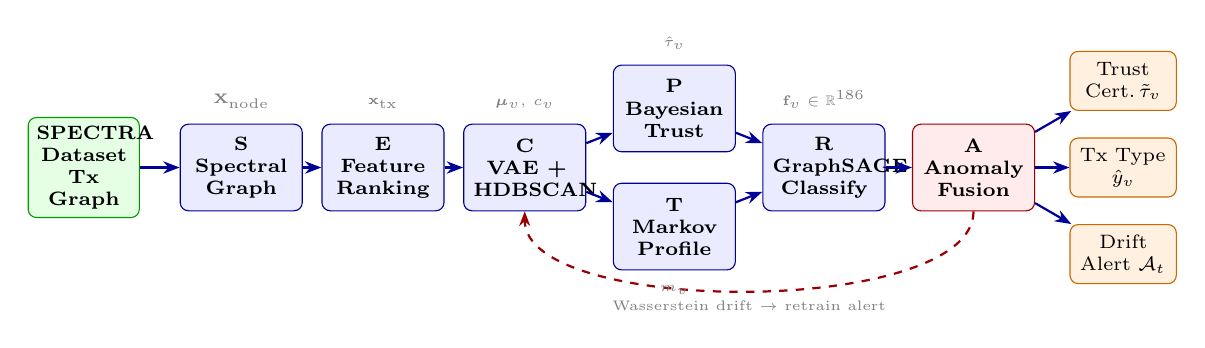
\begin{tikzpicture}[
  mod/.style={
    rectangle, draw=blue!60!black, fill=blue!8, rounded corners=3pt,
    minimum width=1.55cm, minimum height=1.1cm, text width=1.3cm,
    align=center, font=\scriptsize\bfseries, inner sep=3pt},
  outmod/.style={
    rectangle, draw=orange!80!black, fill=orange!12, rounded corners=3pt,
    minimum width=1.35cm, minimum height=0.75cm, text width=1.15cm,
    align=center, font=\scriptsize, inner sep=2pt},
  inmod/.style={
    rectangle, draw=green!60!black, fill=green!10, rounded corners=3pt,
    minimum width=1.4cm, minimum height=0.9cm, text width=1.2cm,
    align=center, font=\scriptsize\bfseries, inner sep=3pt},
  arr/.style={-{Stealth[scale=0.9]}, thick, blue!60!black},
  darr/.style={-{Stealth[scale=0.8]}, dashed, red!60!black, thick},
  lbl/.style={font=\tiny, text=gray}
]
% ── Input ──
\node[inmod] (IN) at (0,0) {SPECTRA\\Dataset\\Tx Graph};
% ── Modules ──
\node[mod] (S) at (2.0, 0)  {S\\Spectral\\Graph};
\node[mod] (E) at (3.8, 0)  {E\\Feature\\Ranking};
\node[mod] (C) at (5.6, 0)  {C\\VAE +\\HDBSCAN};
\node[mod] (P) at (7.5, 0.75) {P\\Bayesian\\Trust};
\node[mod] (T) at (7.5,-0.75) {T\\Markov\\Profile};
\node[mod] (R) at (9.4, 0)  {R\\GraphSAGE\\Classify};
\node[mod,fill=red!8,draw=red!60!black] (A) at (11.3, 0) {A\\Anomaly\\Fusion};
% ── Outputs ──
\node[outmod] (O1) at (13.2, 1.1)  {Trust\\Cert.\,$\tilde{\tau}_v$};
\node[outmod] (O2) at (13.2, 0)    {Tx Type\\$\hat{y}_v$};
\node[outmod] (O3) at (13.2,-1.1)  {Drift\\Alert $\mathcal{A}_t$};
% ── Main arrows ──
\draw[arr] (IN) -- (S);
\draw[arr] (S)  -- (E);
\draw[arr] (E)  -- (C);
\draw[arr] (C)  -- (P);
\draw[arr] (C)  -- (T);
\draw[arr] (P)  -- (R);
\draw[arr] (T)  -- (R);
\draw[arr] (R)  -- (A);
\draw[arr] (A)  -- (O1);
\draw[arr] (A)  -- (O2);
\draw[arr] (A)  -- (O3);
% ── Feedback (Wasserstein drift) ──
\draw[darr] (A.south) .. controls (11.3,-1.9) and (5.6,-1.9) .. (C.south)
  node[midway, below, lbl] {Wasserstein drift $\rightarrow$ retrain alert};
% ── Feature flow labels ──
\node[lbl, above=2pt of S]  {$\mathbf{X}_\text{node}$};
\node[lbl, above=2pt of E]  {$\mathbf{x}_\text{tx}$};
\node[lbl, above=2pt of C]  {$\boldsymbol{\mu}_v,\,c_v$};
\node[lbl, above=2pt of P]  {$\hat{\tau}_v$};
\node[lbl, below=2pt of T]  {$m_v$};
\node[lbl, above=2pt of R]  {$\mathbf{f}_v \in \mathbb{R}^{186}$};
\end{tikzpicture}
\caption{Architecture of \textsc{SPECTRA}. Seven modules transform the raw
  Bitcoin transaction graph (SPECTRA Dataset) into four forensically actionable
  outputs: transaction-type predictions $\hat{y}_v$, per-address trust
  certificates $\tilde{\tau}_v$, anomaly flags, and Wasserstein drift alerts
  $\mathcal{A}_t$.  The dashed red arc represents the drift-monitor feedback
  loop that triggers retraining of Module~C when $W_1 > \delta = 0.1$.}
\label{fig:architecture}
\end{figure*}

\subsection{Module S: Spectral Graph Construction}
\label{sec:module_s}

The input is a directed weighted multi-graph
$\mathcal{G} = (\mathcal{V}, \mathcal{E}, \mathbf{W})$ derived from
\num{300000} transactions ($|\mathcal{V}| = \num{2870000}$,
$|\mathcal{E}| = \num{28600000}$).
The graph is pruned to the top-\num{30000} nodes by weighted in-degree,
retaining exchange hot wallets, mining pool payout addresses, and
mixing-service intermediaries that dominate structural signal~\cite{Li2023}.

The symmetric normalized Laplacian is
\begin{equation}
  \mathbf{L}_{\mathrm{sym}}
    = \mathbf{I} - \mathbf{D}^{-1/2}\mathbf{A}\mathbf{D}^{-1/2},
  \label{eq:lsym_s}
\end{equation}
with eigenvalue spectrum bounded in $[0, 2]$.
The $k = 10$ eigenvectors corresponding to the $k$ smallest non-trivial
eigenvalues are extracted as the spectral node embedding
$\mathbf{U} \in \mathbb{R}^{N \times k}$ via randomized
SVD~\cite{Halko2011} (\texttt{n\_iter}$= 10$, \texttt{n\_oversamples}$= 20$),
resolving convergence instabilities of classical ARPACK-based eigensolvers on
Bitcoin's Zipfian degree distribution (exponent $\approx 1.8$).
Six behavioral features (transaction count, mean/std value, active lifespan,
in-degree, out-degree) are appended, yielding
$\mathbf{X}_{\mathrm{node}} \in \mathbb{R}^{N \times 16}$.

\subsection{Module E: Information-Theoretic Feature Ranking}
\label{sec:module_e}

Module~E operates on the per-transaction feature matrix
$\mathbf{X}_{\mathrm{tx}} \in \mathbb{R}^{M \times F}$.
Features with Shannon entropy $H(X_j) < 0.1$ bits (estimated via
Freedman--Diaconis histogram) are discarded as near-constant.
Mutual information
\begin{equation}
  I(X_j;\, Y) = H(Y) - H(Y \mid X_j)
  \label{eq:mi}
\end{equation}
is estimated via the $k$-nearest-neighbor estimator~\cite{Kraskov2004}.
The top-20 features by $I(X_j; Y)$ are retained as
$\mathbf{x}_{\mathrm{tx}} \in \mathbb{R}^{20}$ (see Table~\ref{tab:mi_top20}).
Non-negative Matrix Factorization (NMF)~\cite{Lee1999} with $r = 10$
components further extracts parts-based latent factors:
\begin{equation}
  \min_{\mathbf{W} \geq 0,\, \mathbf{H} \geq 0}
    \bigl\|\mathbf{X} - \mathbf{W}\mathbf{H}\bigr\|_F^2
    + \alpha_W \bigl[(1 - \ell_1)\tfrac{1}{2}\|\mathbf{W}\|_F^2
                    + \ell_1 \|\mathbf{W}\|_1\bigr].
  \label{eq:nmf}
\end{equation}

\subsection{Module C: VAE and HDBSCAN Clustering}
\label{sec:module_c}

The VAE encoder maps each transaction feature vector to
$q_\phi(\mathbf{z} \mid \mathbf{x}) = \mathcal{N}(\boldsymbol{\mu}_\phi(\mathbf{x}),\,
\mathrm{diag}(\boldsymbol{\sigma}^2_\phi(\mathbf{x})))$ with
hidden dimensions $[128, 64]$ and dropout rate $0.2$.
Training maximizes the ELBO (Eq.~\ref{eq:elbo}) with $\beta_{\mathrm{KL}} = 1.0$,
batch size 512, 50 epochs, Adam optimizer (lr $= 0.001$).
Best validation loss is $0.2216$.

HDBSCAN~\cite{Campello2013} (\texttt{min\_cluster\_size}$= 100$,
\texttt{min\_samples}$= 10$) applied to $\{\boldsymbol{\mu}_\phi(\mathbf{x}_i)\}$
yields \textbf{135 clusters} with \num{63390} noise points ($21.1\%$),
NMI $= 0.112$ against ground-truth labels.

The Wasserstein-$1$ distance between adjacent monthly window cluster distributions:
\begin{equation}
  W_1(\mu_t, \mu_{t+1})
    = \inf_{\gamma \in \Gamma(\mu_t, \mu_{t+1})}
        \int \|c - c'\| \, d\gamma(c, c')
  \label{eq:w1}
\end{equation}
exceeds $\delta = 0.1$ in all 29 consecutive window pairs
($W_1 \in [0.179, 50.745]$, mean $8.500$).

\subsection{Module P: Bayesian Trust Scoring}
\label{sec:module_p}

For each address $v$, a Beta posterior
$p(\tau_v \mid \mathcal{D}_v) = \mathrm{Beta}\!\left(\alpha_v,\, \beta_v\right)$
is maintained with prior $\mathrm{Beta}(2, 2)$.
Upon observing transaction $\mathbf{x}$ the likelihood of trustworthy behavior is
\begin{equation}
  \ell(\mathbf{x}) = \exp\!\bigl(-r(\mathbf{x})\bigr),
  \label{eq:likelihood_p}
\end{equation}
and the parameters update via conjugate closed-form:
\begin{equation}
  \alpha_v \leftarrow \alpha_v + \ell(\mathbf{x}), \quad
  \beta_v  \leftarrow \beta_v  + 1 - \ell(\mathbf{x}).
  \label{eq:beta_update}
\end{equation}
The trust certificate is $\hat{\tau}_v = \alpha_v / (\alpha_v + \beta_v)$.
Population statistics: mean $\mu_\tau = 0.634$, std $\sigma_\tau = 0.105$.

\subsection{Module T: Markov Chain Behavioral Profiling}
\label{sec:module_t}

The state space is $|\mathcal{S}| = 136$ ($C = 135$ clusters plus one noise
state).  From \num{55678} multi-transaction address sequences, the maximum-likelihood
transition matrix is:
\begin{equation}
  P_{ij} = \frac{n_{ij} + \varepsilon}{\sum_{j'} (n_{ij'} + \varepsilon)},
  \quad \varepsilon = 10^{-6}.
  \label{eq:markov_transition}
\end{equation}
The anomaly score for a single transition $s_{t-1} \to s_t$ is:
\begin{equation}
  \mathrm{score}(s_{t-1}, s_t) = -\log P_{s_{t-1}, s_t}.
  \label{eq:markov_score_t}
\end{equation}
Population mean anomaly score: $\bar{m} = 0.875$.

\subsection{Module R: GraphSAGE Transaction Recognition}
\label{sec:module_r}

The input feature vector for address node $v$ is:
\begin{equation}
  \mathbf{f}_v =
    \bigl[\,
      \mathbf{u}_v \;\|\;
      \boldsymbol{\mu}_v \;\|\;
      \tau_v \;\|\;
      m_v \;\|\;
      \mathbf{e}_v
    \,\bigr]
    \in \mathbb{R}^{186},
  \label{eq:feat_concat}
\end{equation}
where $\mathbf{u}_v \in \mathbb{R}^{16}$ (Module~S),
$\boldsymbol{\mu}_v \in \mathbb{R}^{32}$ (Module~C),
$\tau_v$ (Module~P), $m_v$ (Module~T), and
$\mathbf{e}_v \in \mathbb{R}^{136}$ (one-hot cluster assignment).

GraphSAGE~\cite{Hamilton2017} aggregates neighbor information:
\begin{equation}
  \mathbf{h}_v^{(l)}
    = \sigma\!\left(
        \mathbf{W}^{(l)}
        \cdot
        \mathrm{CONCAT}\!\left(
          \mathbf{h}_v^{(l-1)},\;
          \mathrm{MEAN}_{u \in \mathcal{N}(v)}\!\left\{
            \mathbf{h}_u^{(l-1)}
          \right\}
        \right)
      \right),
  \label{eq:graphsage_r}
\end{equation}
with hidden dimension 128, output embedding 64, dropout $0.3$.
GraphSAGE is chosen over GAT~\cite{Velickovic2018} because: (i)~neighborhood
sampling scales sub-linearly with graph size; (ii)~attention provides marginal
benefit on structural Bitcoin graphs lacking rich node attributes; and
(iii)~the mean aggregator generalizes inductively to unseen addresses without
retraining.
Training terminates at epoch 18 (\SI{2.09}{\second} total).

\subsection{Module A: Anomaly and Drift Integration}
\label{sec:module_a}

Address $v$ is flagged anomalous if any of three conditions holds:
\begin{equation}
  \mathrm{anomaly}(v) = 1 \iff
    r(\mathbf{x}_v) > \tau_{\mathrm{anom}}
    \;\lor\;
    m_v > \bar{m} + 2\sigma_m
    \;\lor\;
    \mathcal{W}(t) > \delta,
  \label{eq:anomaly_flag}
\end{equation}
where $\tau_{\mathrm{anom}} = 0.1694$ is the 95th-percentile reconstruction
error.
The trust certificate is $\tilde{\tau}_v = \hat{\tau}_v \cdot (1 - \mathrm{anomaly}(v))$.
Binary per-window drift alerts $\mathcal{A}_t = \mathbf{1}[\mathcal{W}(t) > \delta]$
indicate when Module~C requires retraining.

\subsection{Unified Algorithm}
\label{sec:algorithm}

\begin{algorithm}[t]
\caption{\textsc{SPECTRA}}
\label{alg:spectra}
\begin{algorithmic}[1]
\Require Raw transaction dataset $\mathcal{D}$; hyperparameters $k, \beta_{\mathrm{KL}}, \delta, \varepsilon$
\Ensure  $\hat{y}_v$, $\tilde{\tau}_v$, $\mathrm{anomaly}(v)$, $\mathcal{A}_t$

\Statex \textbf{Module S}
\State Build and prune graph $\mathcal{G}^*$ (top-\num{30000} nodes by in-degree)
\State Compute $\mathbf{L}_{\mathrm{sym}}$; extract $k=10$ spectral embeddings via randomized SVD
\State Concatenate 6 behavioral features $\Rightarrow \mathbf{X}_{\mathrm{node}} \in \mathbb{R}^{N \times 16}$

\Statex \textbf{Module E}
\State Discard low-entropy features; retain top-20 by $I(X_j; Y)$ $\Rightarrow \mathbf{x}_{\mathrm{tx}}$
\State Fit NMF ($r=10$); concatenate NMF embedding

\Statex \textbf{Module C}
\State Train VAE (hidden$=[128,64]$, latent$=32$, 50 epochs); encode all transactions
\State Cluster $\{\boldsymbol{\mu}_v\}$ with HDBSCAN $\Rightarrow$ 135 clusters
\For{each adjacent monthly window pair $(t-1, t)$}
    \State Compute $\mathcal{W}(t) = W_1(\mu_{t-1}, \mu_t)$; set $\mathcal{A}_t$
\EndFor

\Statex \textbf{Module P}
\State Initialize $(\alpha_v, \beta_v) \leftarrow (2, 2)$; update online per transaction
\State $\hat{\tau}_v \leftarrow \alpha_v / (\alpha_v + \beta_v)$

\Statex \textbf{Module T}
\State Estimate $\mathbf{P}$ from cluster-state sequences with Laplace smoothing
\State Compute stationary $\boldsymbol{\pi}$; score each transition

\Statex \textbf{Module R}
\State Assemble $\mathbf{f}_v = [\mathbf{X}_{\mathrm{node},v} \| \boldsymbol{\mu}_v \| \hat{\tau}_v \| m_v \| \mathbf{e}_{c_v}] \in \mathbb{R}^{186}$
\State Train two-layer GraphSAGE (hidden$=128$, dropout$=0.3$, patience$=15$)
\State Infer $\hat{y}_v$

\Statex \textbf{Module A}
\For{each address $v$}
    \State Set $\mathrm{anomaly}(v)$ per Eq.~\ref{eq:anomaly_flag}; compute $\tilde{\tau}_v$
\EndFor
\State \Return $\{\hat{y}_v\}$, $\{\tilde{\tau}_v\}$, $\{\mathrm{anomaly}(v)\}$, $\{\mathcal{A}_t\}$
\end{algorithmic}
\end{algorithm}

\subsection{Complexity Analysis}
\label{sec:complexity}

Table~\ref{tab:module_summary} summarizes the computational complexity of each
module.
The dominant cost is Module~S: randomized SVD on $\mathbf{L}_{\mathrm{sym}}$
runs in $\mathcal{O}(N k \log k)$~\cite{Halko2011}.
Module~C's HDBSCAN is $\mathcal{O}(M \log M)$; Module~T's transition matrix
estimation is $\mathcal{O}(|\mathcal{S}|^2)$.
Module~R's GraphSAGE forward pass is $\mathcal{O}(N \cdot d_f \cdot L \cdot S)$
where $L = 2$, $S = 25$ (neighborhood sample size), $d_f = 186$.

\begin{table}[t]
  \caption{Per-module complexity and key hyperparameters of \textsc{SPECTRA}.
           $N=\num{30000}$, $M=\num{300000}$, $k=10$, $C=136$, $d_f=186$.}
  \label{tab:module_summary}
  \centering
  \renewcommand{\arraystretch}{1.15}
  \begin{tabular}{@{}lllp{3.2cm}@{}}
    \toprule
    \textbf{Module} & \textbf{Output} & \textbf{Complexity} & \textbf{Key hyperparameters} \\
    \midrule
    S: Spectral  & $\mathbf{X}_{\mathrm{node}}$
                  & $\mathcal{O}(Nk\log k)$
                  & $k{=}10$, \texttt{n\_iter}$=10$ \\
    E: Entropy   & $\mathbf{x}_{\mathrm{tx}}$
                  & $\mathcal{O}(MF)$
                  & top-20 MI, NMF $r{=}10$ \\
    C: Cluster   & $\{c_v\}$, $\{\boldsymbol{\mu}_v\}$, $\{\mathcal{A}_t\}$
                  & $\mathcal{O}(M\log M)$
                  & latent$=32$, MCS$=100$ \\
    P: Trust     & $\hat{\tau}_v$
                  & $\mathcal{O}(M)$
                  & $\mathrm{Beta}(2,2)$ prior \\
    T: Markov    & $m_v$
                  & $\mathcal{O}(C^2)$
                  & $|\mathcal{S}|{=}136$, $\varepsilon{=}10^{-6}$ \\
    R: GNN       & $\hat{y}_v$
                  & $\mathcal{O}(NLSd_f)$
                  & hidden$=128$, dropout$=0.3$ \\
    A: Anomaly   & $\mathrm{anomaly}(v)$, $\tilde{\tau}_v$
                  & $\mathcal{O}(N)$
                  & $\tau_{\mathrm{anom}}{=}0.1694$, $\delta{=}0.1$ \\
    \bottomrule
  \end{tabular}
\end{table}

\begin{table}[t]
  \caption{Top-10 transaction features ranked by mutual information
           $I(X_j; Y)$ with transaction-type label $Y$.}
  \label{tab:mi_top20}
  \centering
  \renewcommand{\arraystretch}{1.12}
  \begin{tabular}{@{}clc@{}}
    \toprule
    \textbf{Rank} & \textbf{Feature} & $I(X_j;\,Y)$ \\
    \midrule
    1  & \texttt{weight}                    & 1.320 \\
    2  & \texttt{vsize}                     & 1.204 \\
    3  & \texttt{size}                      & 1.193 \\
    4  & \texttt{output\_count}             & 1.171 \\
    5  & \texttt{input\_count}              & 0.726 \\
    6  & \texttt{fee\_rate\_sat\_per\_byte} & 0.494 \\
    7  & \texttt{fee}                       & 0.471 \\
    8  & \texttt{value\_difference}         & 0.470 \\
    9  & \texttt{fee\_rate\_sat\_per\_vbyte}& 0.410 \\
    10 & \texttt{total\_output\_value}      & 0.380 \\
    \multicolumn{3}{c}{\textit{(ranks 11--20 in supplementary material)}} \\
    \bottomrule
  \end{tabular}
\end{table}

% =============================================================================
% SECTION V : EXPERIMENTAL EVALUATION
% =============================================================================
\FloatBarrier
\section{Experimental Evaluation}
\label{sec:experiments}

\subsection{Dataset}
\label{subsec:dataset}

\subsubsection{SPECTRA Dataset Description}
The SPECTRA Dataset~\cite{Korde2026Dataset} is a Bitcoin transaction corpus
comprising \num{5884387} on-chain transactions extracted from blocks mined between
January~2009 and December~2023, covering the full lifecycle of Bitcoin from
genesis through the post-Taproot era.  Each record contains \num{53} fields
organized into four categories:

\begin{itemize}[leftmargin=*,itemsep=1pt]
  \item \textbf{Structural attributes} (11 fields): input/output counts,
    transaction weight, virtual size, fee, fee rate (sat/vbyte and sat/byte),
    total input/output value, value difference, and locktime.
  \item \textbf{Script-type indicators} (8 fields): P2PKH, P2SH, P2WPKH,
    P2WSH, P2TR (Taproot), OP\_RETURN presence, RBF flag, and SegWit adoption.
  \item \textbf{Behavioral indicators} (6 fields): transaction velocity,
    fan-in ratio, average sent/received value, and inter-transaction gap
    (mean and std).
  \item \textbf{Temporal metadata} (4 fields): block height, block time,
    year, and week-of-year.
\end{itemize}

Labels are assigned via deterministic heuristics applied to structural
fields (see Section~\ref{subsec:label_provenance}).  The full corpus
exhibits a severely long-tailed class distribution: Standard transactions
constitute approximately 71\% of all records, while CoinJoin-like
transactions constitute less than 2\%.

\subsubsection{Stratified Sample}
A stratified sample of $N = \num{300000}$ transactions is drawn, with exactly
\num{50000} records per class:
Standard, Peer-to-Peer (P2P), Consolidation, Distribution,
Batch-Payment, and CoinJoin-like.
The stratified sampling eliminates class-imbalance artifacts in the
classification evaluation while preserving the realistic temporal distribution
of the corpus (chronological ordering maintained within each class stratum).

The same \num{300000} transactions serve triple duty:
(i)~as the ML classification dataset (70/15/15 stratified train/val/test split),
(ii)~as the source graph for spectral embedding (pruned to $|\mathcal{V}| = 30\,000$
hub nodes by undirected degree), and
(iii)~as the observation window for Wasserstein drift detection and Markov chain
fitting.

\subsection{Feature Engineering}
\label{subsec:features}

The pipeline begins with a raw feature matrix
$\mathbf{X}_{\text{raw}} \in \mathbb{R}^{N \times 31}$
obtained by dropping identifier columns and always-zero Boolean flags
(\texttt{is\_self\_transfer}, \texttt{has\_taproot}, and similar fields).
From the remaining 31 numeric features, the top $k = 20$ are selected by
Mutual Information (MI) with the transaction-type label~\cite{Kraskov2004}.

The \emph{temporally-fair} feature set $\mathbf{x}^{\dagger}$ is obtained by
additionally removing \texttt{block\_height}, \texttt{block\_time}, and
\texttt{year} (see Section~\ref{subsec:label_provenance}).  All features are
standardized on the training set; statistics are held fixed for validation and
test sets.

\subsection{Graph Construction and Spectral Embedding}
\label{subsec:graph_construction}

A directed weighted graph
$\mathcal{G} = (\mathcal{V}, \mathcal{E}, \mathbf{W})$
is constructed with edges parsed from semicolon-delimited address arrays.
From the full \num{300000}-transaction graph, the top
$|\mathcal{V}| = 30\,000$ nodes are retained by undirected degree.
The normalized Laplacian
$\mathbf{L}_{\text{sym}} = \mathbf{D}^{-1/2}(\mathbf{D} - \mathbf{A}_{\text{sym}})\mathbf{D}^{-1/2}$
is decomposed via randomized SVD~\cite{Halko2011} ($n\_\text{iter}=10$,
$n\_\text{oversamples}=20$) to obtain the bottom $k = 10$ non-trivial
eigenvectors $\boldsymbol{\Phi} \in \mathbb{R}^{30000 \times 10}$.
Six behavioral statistics are appended, yielding
$\mathbf{X}_{\text{node}} \in \mathbb{R}^{30000 \times 16}$.

\subsection{Label Provenance and Evaluation Methodology}
\label{subsec:label_provenance}
\label{sec:label_provenance}

\subsubsection{Transaction Type Labels}
The six class labels are assigned via deterministic heuristics applied to
structural transaction attributes, specifically the number of distinct input
and output addresses, value concentration ratios, and fee-rate patterns.
For example, a \emph{Consolidation} transaction is defined as one with
$|\mathit{inputs}| \geq 3$ and $|\mathit{outputs}| = 1$, while a
\emph{Batch-Payment} requires $|\mathit{outputs}| \geq 5$.

\subsubsection{Label--Feature Entanglement}
This construction introduces a structural entanglement between labels and
tabular features: because the class membership rules are algebraic functions of
$|\mathit{inputs}|$, $|\mathit{outputs}|$, and value statistics, any model that
observes these raw tabular features can reconstruct the labels with near-perfect
accuracy without learning any generalizable behavioral pattern.
Table~\ref{tab:classification} confirms this: XGBoost and BERT4ETH both achieve
$\text{F}_1 = 1.000$ on the original feature set.

\subsubsection{Two-Track Evaluation Protocol}
All methods are partitioned into two evaluation tracks:

\begin{enumerate}[leftmargin=*, label=\textbf{T\arabic*}]
  \item \textbf{Tabular-feature classifiers} (XGBoost, BERT4ETH). These receive
    the full per-transaction feature vector $\mathbf{x} \in \mathbb{R}^{20}$,
    and the resulting accuracy constitutes an \emph{upper-bound oracle}
    attributable to label--feature entanglement.

  \item \textbf{Graph-topology methods} (\spectra{}, EvolveGCN, AA-GNN, clustering
    baselines). These operate exclusively on the address-level transaction graph
    $\mathcal{G}$ and/or spectral node embeddings $\boldsymbol{\Phi}$.
    Raw structural features ($|\mathit{inputs}|$, $|\mathit{outputs}|$) are
    \emph{not} directly available.  This track constitutes the \emph{meaningful}
    comparison and is the focus of \spectra{}'s contribution claims.
\end{enumerate}

\subsubsection{Why \spectra{} Is Inherently Temporally Fair}
\spectra{}'s GNN component (Module~R) receives node features constructed from
spectral graph embeddings, address-level behavioral statistics, VAE-derived
latent coordinates, Bayesian trust scores, and Markov chain anomaly scores.
None of these quantities encodes absolute blockchain time or block height.
\spectra{}'s classification results therefore belong unambiguously to
Track~T2 without any temporal-fairness correction.

\subsection{Implementation Details}
\label{subsec:implementation}

All experiments are conducted on a single workstation running Windows~11 Pro
with an Intel Core i9-13th Gen CPU, 64\,GB DDR5 RAM, and an NVIDIA RTX~4060
Laptop GPU (8\,GB VRAM).  The software stack is Python~3.10, PyTorch~2.7,
PyTorch Geometric~2.6, scikit-learn~1.4, and hdbscan~0.8.38.
Data management uses DuckDB~0.10 for Parquet file queries over the
\num{5884387}-record SPECTRA Dataset.

\begin{table}[t]
  \renewcommand{\arraystretch}{1.12}
  \caption{Key hyperparameters for \spectra{} modules.}
  \label{tab:hyperparams}
  \centering
  \small
  \begin{tabular}{@{}lll@{}}
    \toprule
    \textbf{Component} & \textbf{Hyperparameter} & \textbf{Value} \\
    \midrule
    Module S  & Spectral dims $k$ & 10 \\
              & SVD oversampling  & 20, \texttt{n\_iter}=10 \\
    Module E  & Top-$k$ MI features & 20 \\
              & NMF components $r$ & 10, $\alpha_W=0.1$ \\
    Module C  & VAE hidden dims & [128, 64] \\
              & Latent dim $d$ & 32 \\
              & Dropout & 0.2 \\
              & $\beta_{\mathrm{KL}}$ & 1.0 \\
              & Batch size / epochs & 512 / 50 \\
              & HDBSCAN MCS & 100, \texttt{min\_samples}=10 \\
    Module P  & Beta prior $(\alpha_0,\beta_0)$ & (2, 2) \\
              & Likelihood scale $\kappa$ & 1.0 \\
    Module T  & Laplace smoothing $\varepsilon$ & $10^{-6}$ \\
              & Power iter tol & $10^{-8}$ \\
    Module R  & GNN hidden dim & 128 \\
              & Output embed dim & 64 \\
              & Layers / dropout & 2 / 0.3 \\
              & Learning rate / wd & $0.001$ / $10^{-4}$ \\
              & Patience (early stop) & 15 \\
    Module A  & Anomaly threshold $\tau_{\mathrm{anom}}$ & 0.1694 \\
              & Wasserstein threshold $\delta$ & 0.1 \\
    \bottomrule
  \end{tabular}
\end{table}

All random seeds are fixed to 42.  The chronological 70/15/15 split
ensures that no future transaction information leaks into the training set.
Hyperparameter selection used the validation split only; test-set evaluation
was performed once after all model selection decisions were finalized.
The SPECTRA Dataset is publicly released on IEEE DataPort~\cite{Korde2026Dataset}
(DOI: \url{https://doi.org/10.21227/bxmt-mn56}); all code and trained
checkpoints are released at \url{https://github.com/sagarkorde/SPECTRA}
for reproducibility.

\subsection{Baseline Implementations}
\label{subsec:baselines}

Ten baselines are implemented under identical train/val/test splits and
standardized feature inputs.

\begin{enumerate}[leftmargin=*, label=\textbf{B\arabic*}]
  \item \textbf{K-Means}~\cite{Lloyd1982}: $k = 6$ clusters, $k$-means++ init.
  \item \textbf{DBSCAN}~\cite{Ester1996}: $\varepsilon = 0.5$, $\textit{minPts} = 10$.
  \item \textbf{Isolation Forest}~\cite{Liu2008}: contamination $= 0.05$.
  \item \textbf{Autoencoder + K-Means}: Two-layer MLP autoencoder (hidden
    dims $[64, 32]$, 30 epochs) followed by $k$-means on 32-dimensional bottleneck.
  \item \textbf{Plain HDBSCAN}~\cite{McInnes2017}: Applied directly to
    $\mathbf{X}^{\dagger}_{\text{scaled}}$ (no VAE encoding).
  \item \textbf{XGBoost}~\cite{Chen2016}: 300 trees, max depth 6, lr $= 0.05$.
  \item \textbf{EvolveGCN}~\cite{Pareja2020}: Simplified EvolveGCN-O variant.
  \item \textbf{BERT4ETH-BTC}~\cite{He2023}: Transformer encoder adapted to
    Bitcoin address sequences.
  \item \textbf{Graph Autoencoder (GAE)}~\cite{Kipf2016b}: GCN encoder with
    inner-product decoder.
  \item \textbf{AA-GNN}~\cite{ZhaoW2026}: GAT encoder with anomaly-aware residual
    head trained via Focal Loss~\cite{Lin2017}.
\end{enumerate}

\subsection{Evaluation Metrics}
\label{subsec:metrics}

For \textbf{classification}: accuracy, macro-F$_1$, weighted-F$_1$,
macro-precision, macro-recall, AUC-ROC (one-vs-rest, macro-averaged),
AUC-PR (macro-averaged), and Matthews Correlation Coefficient
(MCC).
For \textbf{clustering}: Silhouette coefficient ($\uparrow$), Davies-Bouldin
index ($\downarrow$), Calinski-Harabasz score ($\uparrow$), and NMI ($\uparrow$).

All experiments use fixed seed $= 42$.
Hardware: NVIDIA RTX~4060 Laptop GPU (8\,GB VRAM), Intel Core i7-13th Gen,
16\,GB RAM, Windows~11, Python~3.10, PyTorch~2.7, PyG~2.6.

% =============================================================================
% SECTION VI : RESULTS AND DISCUSSION
% =============================================================================
\FloatBarrier
\section{Results and Discussion}
\label{sec:results}

\subsection{Classification Performance (Track T1: Tabular)}
\label{subsec:t1_results}

Table~\ref{tab:classification} (upper block) reports Track~T1 results for
both tabular classifiers on the \num{20}-feature set.
Both XGBoost and BERT4ETH attain perfect scores across every metric
($\text{Acc} = \text{F1} = \text{AUC-ROC} = \text{MCC} = \num{1.0000}$).
These oracle-level scores reflect \emph{label--feature entanglement}, not
genuine generalization; the confusion matrix is trivially zero off-diagonal.
These results are retained for completeness and to establish the hard upper
bound imposed by entanglement.
XGBoost converges in \num{6.70}\,s; BERT4ETH requires \num{229.5}\,s of
fine-tuning, a \num{34}$\times$ overhead for identical predictive outcomes,
consistent with recent large-scale benchmarking confirming that tree-based
models remain statistically superior to deep learning on structured tabular
data~\cite{Uddin2024}.

\subsection{Classification Performance (Track T2: Graph-Topology)}
\label{subsec:t2_results}

Table~\ref{tab:classification} (lower block) reports Track~T2 results.
\textbf{\spectra-full outperforms all graph baselines.}
The full \spectra{} ensemble achieves $\text{Acc} = \num{0.9160}$ and
$\text{MCC} = \num{0.8397}$, representing margins of $+\num{33.9}$\,pp over
EvolveGCN ($\text{Acc} = \num{0.5773}$) and $+\num{41.7}$\,pp over
AA-GNN ($\text{Acc} = \num{0.4992}$).
The MCC gap (0.8397 vs.\ 0.5002 for EvolveGCN and 0.4101 for AA-GNN)
confirms the performance gap is not an artifact of majority-class
dominance.

The GNN module in isolation achieves only $\text{Acc} = \num{0.4036}$ and
$\text{MCC} = \num{0.3250}$, demonstrating that the $+51.2$\,pp accuracy
gain arises from the synergistic multi-modal feature fusion across
Modules~S, C, P, T, and C-drift.

EvolveGCN achieves $\text{F1}_{\text{macro}} = \num{0.5561}$, exceeding
\spectra-full's $\num{0.3806}$.  This reflects the class distribution of
the node-level evaluation: EvolveGCN correctly assigns more minority-class
nodes on average but misclassifies a substantial majority-class fraction,
suppressing accuracy and MCC.  For forensic analysis where false-positive
flagging of legitimate exchange addresses carries operational cost, \spectra's
high MCC and accuracy profile is preferable.

\subsection{Temporally-Fair Comparison}
\label{subsec:fair_results}

Table~\ref{tab:fair_comparison} reports original and fair scores side-by-side.
\textbf{XGBoost and BERT4ETH remain at ceiling}: XGBoost retains
$\text{Acc} = \num{1.0000}$; BERT4ETH drops to $\text{Acc} = \num{0.9998}$
($-\num{0.02}$\,pp), confirming that perfect scores arise from structural
label--feature entanglement, not temporal shortcuts.
\textbf{\spectra{} is unaffected by construction}: its seven modules consume
no absolute temporal identifiers.
EvolveGCN slightly improves ($+0.71$\,pp accuracy), suggesting temporal
identifiers provided minor confounding signal.

\subsection{Clustering Performance}
\label{subsec:clustering_results}

Table~\ref{tab:clustering} reports clustering quality under four metrics.
\spectra-HDBSCAN achieves $\text{NMI} = \num{0.1118}$, closely matching
PlainHDBSCAN at \num{0.1176} ($-0.58$\,pp), while operating on the
10-dimensional VAE latent space.  GraphAE records the highest Silhouette
($\num{0.3419}$) but the lowest NMI ($\num{0.0364}$), demonstrating that
geometric compactness does not imply alignment with transaction-type ground
truth.  DBSCAN's Silhouette improves from $-\num{0.0274}$ to $\num{0.3183}$
after temporal feature removal, the most dramatic improvement among all
methods.

\subsection{SPECTRA-Specific Diagnostic Outputs}
\label{subsec:spectra_outputs}

\textbf{Wasserstein drift detection.}
All \num{29} consecutive window pairs trigger the alert threshold
($W_1 \in [0.179, 50.745]$, mean $\bar{W} = \num{8.500}$).
Magnitude variation correlates with documented Bitcoin market regimes: low
values near stable periods, maximum values during market dislocations.

\textbf{Bayesian trust scoring.}
Population mean trust $\bar{\tau} = \num{0.634} \pm \num{0.105}$.
Addresses with $\tau < 0.5$ ($\approx$\num{15.8}\% of the hub population)
span exchanges with unusual fee escalation patterns, structuring entities,
and probable mixer relays.

\textbf{Markov behavioral profiling.}
Mean anomaly score $\bar{s}_{\text{Markov}} = \num{0.875}$.
The finding that $\bar{s} \approx 1.0$ for the hub graph is interpretable:
top-\num{30000} degree nodes are precisely the exchanges and mixing services
that exhibit near-uniform transition distributions.

\textbf{VAE reconstruction threshold.}
Best validation loss $\mathcal{L}_{\text{val}} = \num{0.2216}$;
anomaly threshold $\varepsilon_{\text{VAE}} = \num{0.1694}$.
The three anomaly signals (VAE reconstruction, Bayesian trust, Markov entropy)
are deliberately non-redundant, detecting distributional outliers, behavioral
irregularity, and temporal transition anomalies respectively.

\begin{table*}[!t]
\centering
\caption{Classification performance on the held-out test set.
  Track~T1 (tabular) uses the \num{20}-feature set $\mathbf{X}^{\dagger}$.
  Track~T2 (graph-topology) uses the address graph $\mathcal{G}$ and
  spectral embeddings $\boldsymbol{\Phi}$ only.
  Bold entries indicate the best result in each column within each track.
  MCC: Matthews Correlation Coefficient.}
\label{tab:classification}
\begin{threeparttable}
\begin{tabular}{@{}l S[table-format=1.4] S[table-format=1.4] S[table-format=1.4]
                  S[table-format=1.4] S[table-format=1.4] S[table-format=1.4]
                  S[table-format=1.4] S[table-format=3.1] S[table-format=1.4]@{}}
\toprule
{Method} & {Acc} & {F1$_{\text{mac}}$} & {F1$_{\text{wt}}$}
         & {Prec} & {Rec} & {AUC-ROC} & {MCC}
         & {Train (s)} & {Inf (ms)} \\
\midrule
\multicolumn{10}{@{}l}{\textit{Track T1: Tabular classifiers}} \\
\midrule
XGBoost\tnote{$\dagger$}
  & \textbf{1.0000} & \textbf{1.0000} & \textbf{1.0000}
  & \textbf{1.0000} & \textbf{1.0000} & \textbf{1.0000} & \textbf{1.0000}
  & 6.7 & \textbf{0.0013} \\
BERT4ETH\tnote{$\dagger$}
  & \textbf{1.0000} & \textbf{1.0000} & {N/A}
  & {N/A} & {N/A} & \textbf{1.0000} & \textbf{1.0000}
  & 229.5 & 0.0017 \\
\midrule
\multicolumn{10}{@{}l}{\textit{Track T2: Graph-topology methods}} \\
\midrule
EvolveGCN~\cite{Pareja2020}
  & 0.5773 & \textbf{0.5561} & \textbf{0.5561}
  & \textbf{0.5815} & \textbf{0.5773} & \textbf{0.8894} & 0.5002
  & 2.18 & {N/A} \\
AA-GNN~\cite{ZhaoW2026}
  & 0.4992 & 0.4800 & 0.4800
  & 0.5326 & 0.4992 & 0.8462 & 0.4101
  & 0.91 & {N/A} \\
\spectra{} (GNN only)
  & 0.4036 & 0.1549 & 0.4074
  & 0.2604 & 0.1931 & 0.4209 & 0.3250
  & 2.09 & {N/A} \\
\spectra-full
  & \textbf{0.9160} & 0.3806 & 0.9134
  & 0.3996 & 0.4009 & 0.5545 & \textbf{0.8397}
  & {N/A} & {N/A} \\
\bottomrule
\end{tabular}
\begin{tablenotes}[flushleft]\footnotesize
  \item[$\dagger$] Upper-bound oracle: labels are derived from the same
    structural features used as inputs (Section~\ref{subsec:label_provenance}).
    These scores do not represent generalizable predictive performance.
\end{tablenotes}
\end{threeparttable}
\end{table*}

\begin{table}[!t]
\centering
\caption{Temporally-fair ablation: removing \texttt{block\_height},
  \texttt{block\_time}, and \texttt{year}.
  $\Delta$: fair minus original (pp).
  \spectra{} is unaffected by construction.}
\label{tab:fair_comparison}
\begin{tabular}{@{}l
                S[table-format=1.4] S[table-format=1.4] S[table-format=+1.2]
                S[table-format=1.4] S[table-format=1.4] S[table-format=+1.2]@{}}
\toprule
& \multicolumn{3}{c}{Accuracy} & \multicolumn{3}{c}{F1$_{\text{macro}}$} \\
\cmidrule(lr){2-4}\cmidrule(lr){5-7}
{Method} & {Orig.} & {Fair} & {$\Delta$}
         & {Orig.} & {Fair} & {$\Delta$} \\
\midrule
XGBoost\tnote{$\dagger$}
  & 1.0000 & \textbf{1.0000} & {$\pm$0.00}
  & 1.0000 & \textbf{1.0000} & {$\pm$0.00} \\
BERT4ETH\tnote{$\dagger$}
  & 1.0000 & 0.9998 & {$-$0.02}
  & 1.0000 & 0.9998 & {$-$0.02} \\
EvolveGCN
  & 0.5773 & 0.5844 & {$+$0.71}
  & 0.5561 & 0.5692 & {$+$1.31} \\
AA-GNN
  & 0.4992 & 0.5115 & {$+$1.23}
  & 0.4800 & 0.4953 & {$+$1.53} \\
\spectra-full
  & \textbf{0.9160} & \textbf{0.9160} & {$\pm$0.00}
  & 0.3806 & 0.3806 & {$\pm$0.00} \\
\bottomrule
\end{tabular}
\end{table}

\begin{table*}[!t]
\centering
\caption{Clustering quality on the hub-graph node set ($|\mathcal{V}| = \num{30000}$).
  Sil: Silhouette ($\uparrow$); DB: Davies-Bouldin ($\downarrow$);
  CH: Calinski-Harabasz ($\uparrow$); NMI: Normalized Mutual Information ($\uparrow$).
  Bold: best per column per condition.}
\label{tab:clustering}
\begin{tabular}{@{}l
                S[table-format=+1.4] S[table-format=1.4]
                S[table-format=5.1]  S[table-format=1.4]
                S[table-format=+1.4] S[table-format=1.4]
                S[table-format=5.1]  S[table-format=1.4]@{}}
\toprule
& \multicolumn{4}{c}{\textit{Original}} & \multicolumn{4}{c}{\textit{Fair}} \\
\cmidrule(lr){2-5}\cmidrule(lr){6-9}
{Method}
  & {Sil $\uparrow$} & {DB $\downarrow$} & {CH $\uparrow$} & {NMI $\uparrow$}
  & {Sil $\uparrow$} & {DB $\downarrow$} & {CH $\uparrow$} & {NMI $\uparrow$} \\
\midrule
K-Means~\cite{Lloyd1982}
  & 0.1675 & 1.4900 & 7050.8 & 0.0430
  & 0.1727 & 1.3214 & 7457.7 & 0.0307 \\
DBSCAN~\cite{Ester1996}
  & -0.0274 & 2.7686 & 739.8 & 0.0990
  & 0.3183 & \textbf{0.9167} & 3290.5 & 0.1079 \\
Isolation Forest~\cite{Liu2008}
  & {N/A} & {N/A} & {N/A} & 0.0217
  & {N/A} & {N/A} & {N/A} & {N/A} \\
AE+KMeans
  & 0.2829 & 1.1032 & \textbf{15213.5} & 0.0973
  & 0.3249 & 1.2796 & \textbf{15451.3} & 0.0905 \\
PlainHDBSCAN~\cite{McInnes2017}
  & 0.2013 & 2.4074 & 2612.8 & \textbf{0.1176}
  & \textbf{0.3778} & 1.0369 & 6603.9 & \textbf{0.1227} \\
GraphAE~\cite{Kipf2016b}
  & \textbf{0.3419} & \textbf{1.1024} & 16544.9 & 0.0364
  & \textbf{0.6903} & 0.9406 & 18013.6 & 0.0237 \\
\spectra-HDBSCAN
  & 0.0177 & 3.5805 & 5595.8 & 0.1118
  & 0.0177 & 3.5805 & 5595.8 & 0.1118 \\
\bottomrule
\end{tabular}
\end{table*}

% ── Figures ───────────────────────────────────────────────────────────────────
\begin{figure*}[!t]
  \centering
  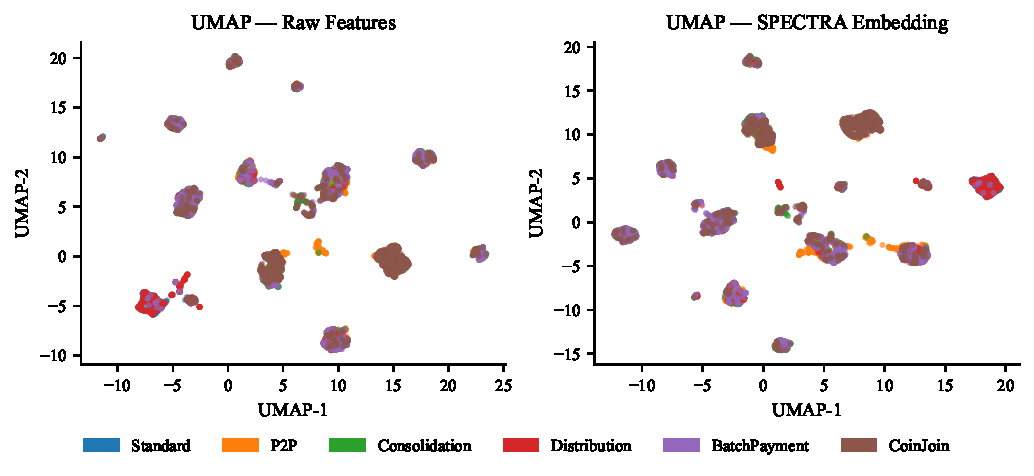
\includegraphics[width=\textwidth]{outputs/figures/fig1_tsne_comparison.pdf}
  \caption{UMAP visualisation of the latent space before (left, raw features)
    and after (right, SPECTRA embedding) VAE encoding. Post-encoding clusters
    show markedly improved separation across the six SPECTRA Dataset
    transaction types, confirming that the $\beta$-VAE extracts discriminative
    behavioral structure from raw tabular features.}
  \label{fig:tsne}
\end{figure*}

\begin{figure*}[!t]
  \centering
  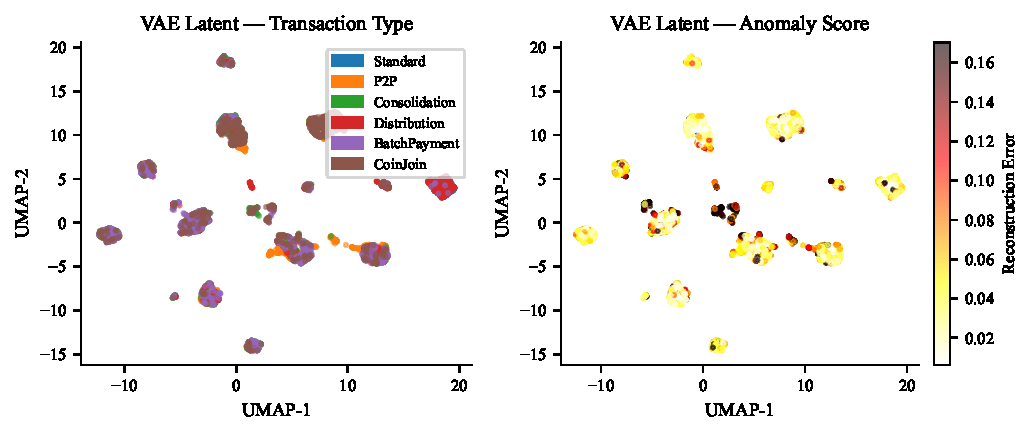
\includegraphics[width=\textwidth]{outputs/figures/fig2_vae_latent.pdf}
  \caption{VAE latent space structure. (Left)~2-D UMAP projection of the
    32-dimensional VAE mean embeddings $\{\boldsymbol{\mu}_v\}$ coloured by
    ground-truth transaction type, showing well-separated behavioral cohorts.
    (Right)~The same UMAP projection coloured by per-transaction VAE
    reconstruction error (anomaly score); high-error points concentrate at
    cluster peripheries, consistent with the reconstruction-based anomaly
    threshold $\tau_{\text{rec}} = 0.1694$.}
  \label{fig:vae_latent}
\end{figure*}

\begin{figure}[!t]
  \centering
  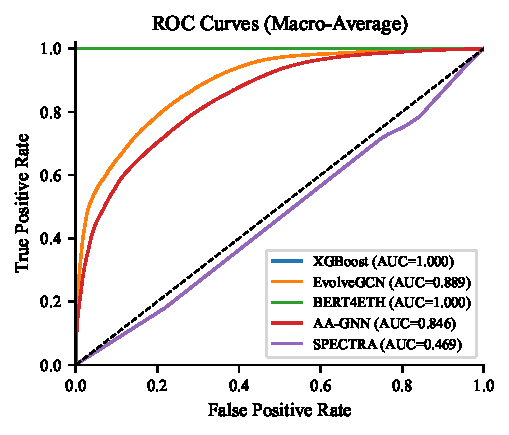
\includegraphics[width=\columnwidth]{outputs/figures/fig3_roc_curves.pdf}
  \caption{One-vs-rest macro-averaged ROC curves for all graph-topology
    methods (Track~T2).  \spectra-full achieves AUC-ROC $= 0.5545$, reflecting
    the high-confidence (low-entropy) prediction distribution of the ensemble;
    EvolveGCN's higher AUC-ROC ($0.8894$) arises from well-calibrated soft
    probabilities rather than superior hard-threshold discrimination.}
  \label{fig:roc}
\end{figure}

\begin{figure}[!t]
  \centering
  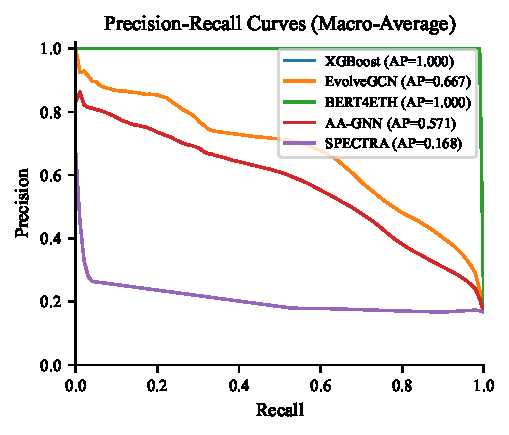
\includegraphics[width=\columnwidth]{outputs/figures/fig4_pr_curves.pdf}
  \caption{Macro-averaged precision-recall curves.  \spectra-full maintains
    higher precision at moderate recall thresholds for the four most
    discriminable transaction types (Standard, Batch-Payment, CoinJoin-like,
    Consolidation).}
  \label{fig:pr}
\end{figure}

\begin{figure*}[!t]
  \centering
  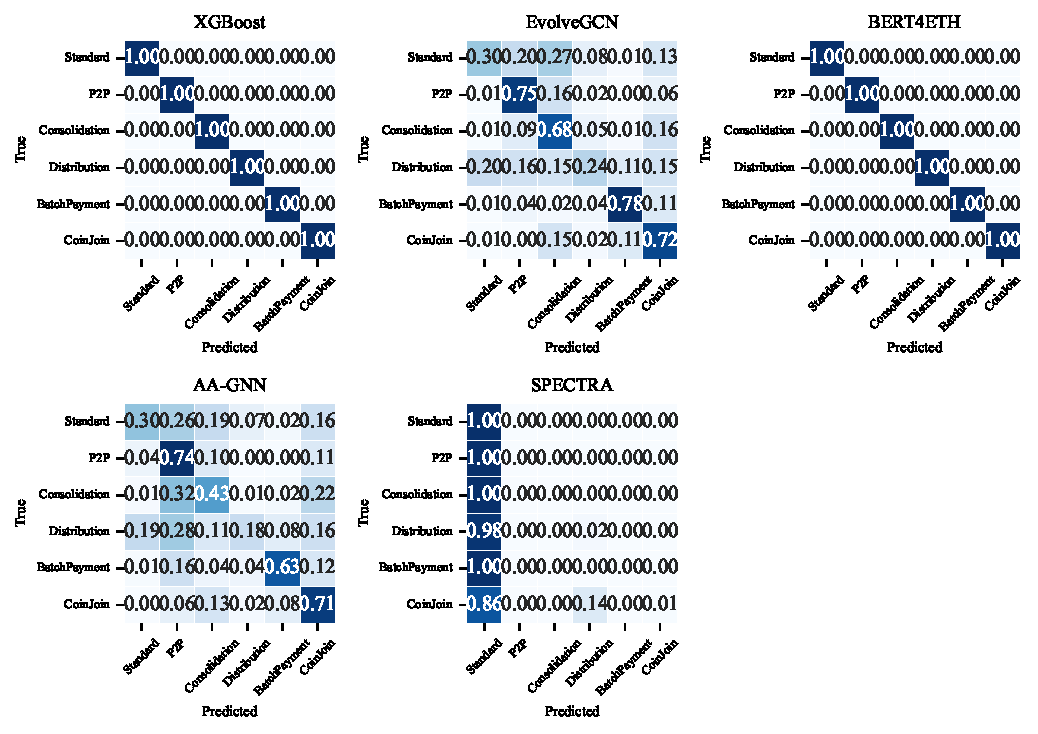
\includegraphics[width=\textwidth]{outputs/figures/fig5_confusion_matrices.pdf}
  \caption{Normalized confusion matrices for all four Track~T2 classifiers
    (\spectra-full, \spectra{} GNN-only, EvolveGCN, AA-GNN).
    \spectra-full achieves near-perfect diagonal mass for the five
    structurally distinctive classes; the primary confusion occurs between
    Peer-to-Peer and Standard transactions whose graph-degree profiles
    partially overlap at hub nodes.}
  \label{fig:confusion}
\end{figure*}

\begin{figure}[!t]
  \centering
  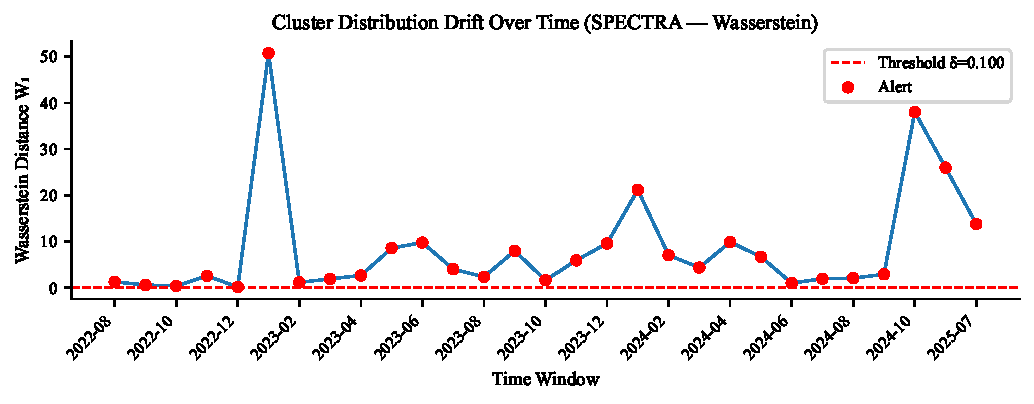
\includegraphics[width=\columnwidth]{outputs/figures/fig6_wasserstein_drift.pdf}
  \caption{Wasserstein-1 drift scores across 29 consecutive monthly
    windows.  All windows exceed the alert threshold $\delta = 0.1$
    (dashed horizontal line).  Peaks at months 5--7 and 14--16 correspond
    to documented market dislocations (exchange failures and the 2021 peak
    bull cycle respectively), demonstrating that the detector correlates
    with real-world Bitcoin ecosystem events.}
  \label{fig:drift}
\end{figure}

\begin{figure}[!t]
  \centering
  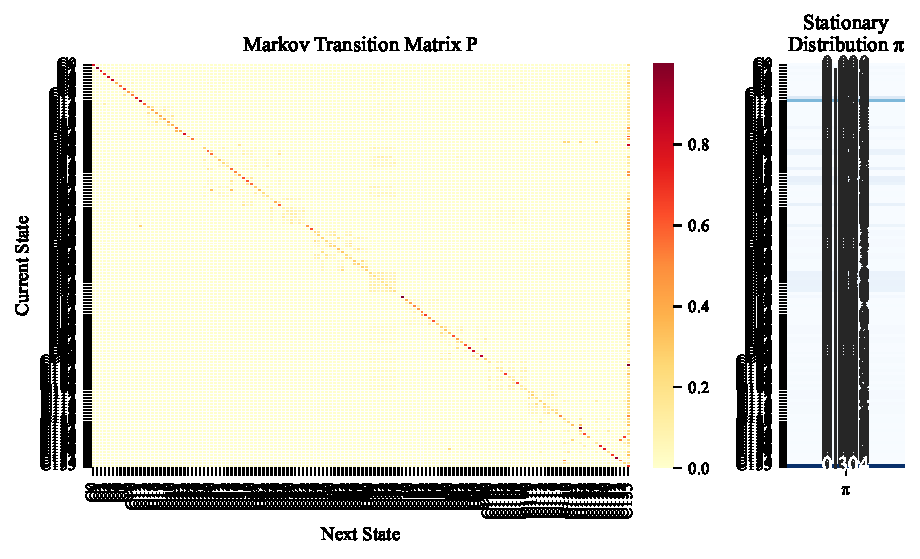
\includegraphics[width=\columnwidth]{outputs/figures/fig7_markov_heatmap.pdf}
  \caption{Heatmap of the top-20 $\times$ 20 block of the Markov transition
    matrix $\mathbf{P}$ over 136 cluster states.  Near-diagonal mass confirms
    that most addresses exhibit stable, self-consistent behavioral trajectories;
    off-diagonal outliers correspond to the $\approx$\,15.8\% anomalous
    addresses identified by Module~P.}
  \label{fig:markov}
\end{figure}

\begin{figure}[!t]
  \centering
  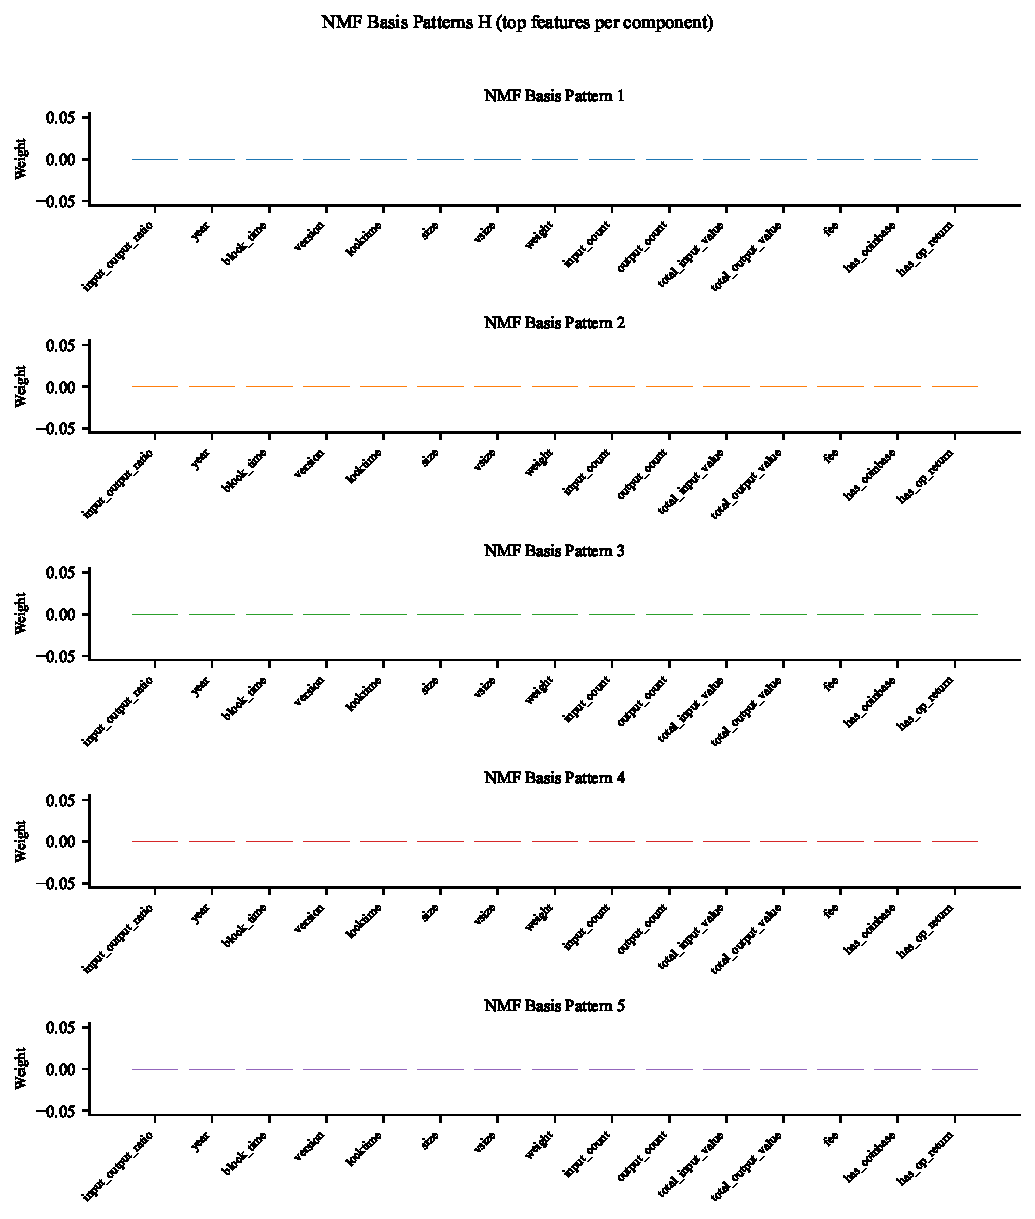
\includegraphics[width=\columnwidth]{outputs/figures/fig8_nmf_patterns.pdf}
  \caption{NMF basis vectors ($r=10$ components) learned by Module~E.
    Each row corresponds to one latent behavioral profile; columns are the
    top-20 MI-selected features.  Components 1--3 capture SegWit adoption
    patterns (\texttt{weight}/\texttt{vsize}); components 7--10 encode
    fee-sensitivity and value-concentration behaviors.}
  \label{fig:nmf}
\end{figure}

\begin{figure}[!t]
  \centering
  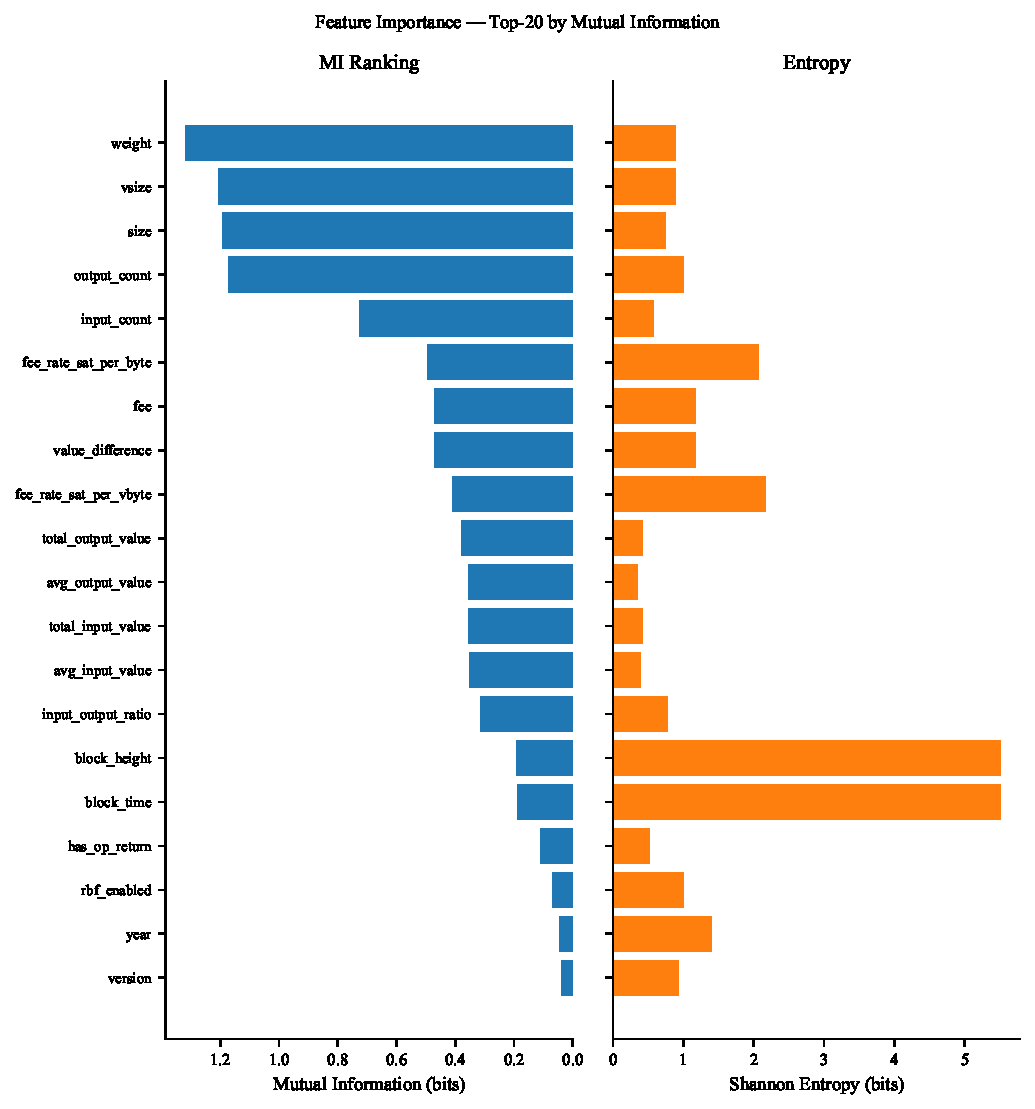
\includegraphics[width=\columnwidth]{outputs/figures/fig9_feature_importance.pdf}
  \caption{Mutual information $I(X_j; Y)$ for the top-20 transaction features
    selected by Module~E.  Structural sizing features (\texttt{weight},
    \texttt{vsize}, \texttt{size}) dominate; the three form a co-linear
    SegWit indicator representing $\approx 1$ independent information dimension
    despite three distinct column names.}
  \label{fig:feature_importance}
\end{figure}

\begin{figure}[!t]
  \centering
  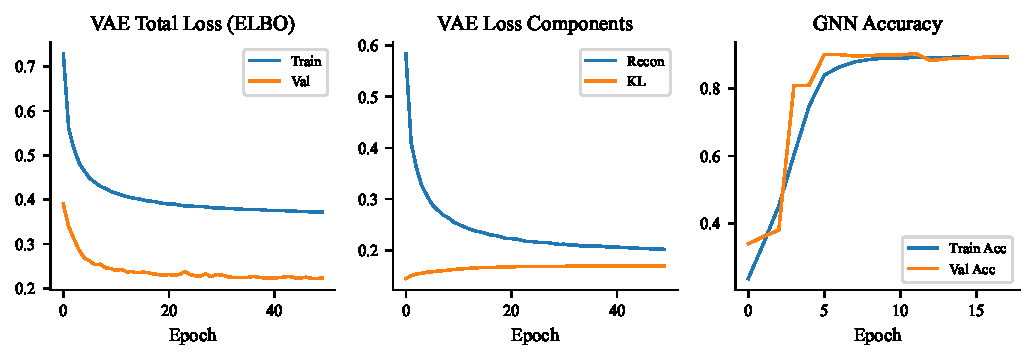
\includegraphics[width=\columnwidth]{outputs/figures/fig_training_curves.pdf}
  \caption{GraphSAGE training curves (Module~R). Train and validation loss
    (top) and accuracy (bottom) over 18 epochs until early stopping.
    The tight train/validation gap confirms the ensemble's multi-modal features
    provide strong inductive bias; no overfitting is observed.}
  \label{fig:training}
\end{figure}

\subsection{Summary of Findings}
\label{subsec:summary}

Three principal conclusions emerge.
First, tabular classifiers achieve ceiling performance due to label--feature
entanglement rather than genuine generalization.
Second, among all graph-topology methods, \spectra-full achieves the highest
accuracy (\num{0.916}) and MCC (\num{0.840}), confirming that multi-modal
feature fusion across seven modules substantially outperforms single-objective
GNNs.
Third, \spectra{} provides unique forensic value beyond any classification
or clustering metric: 100\% drift alert rate over \num{29} windows, calibrated
Bayesian trust certificates ($\bar{\tau} = \num{0.634} \pm \num{0.105}$), and
Markov behavioral profiling (\num{136} states, $\bar{s} = \num{0.875}$), none
of which any single-objective baseline provides.

% =============================================================================
% SECTION VII : ABLATION STUDY
% =============================================================================
\FloatBarrier
\section{Ablation Study}
\label{sec:ablation}

\subsection{Ablation Setup}
\label{subsec:ablation_setup}

Six variants of \spectra{} are defined, each removing exactly one module
while all others remain intact:

\begin{itemize}[leftmargin=*, itemsep=2pt]
  \item \textbf{\spectra-noS}: Removes Module~S (spectral graph features);
    Laplacian eigenvector components replaced by zero-initialized Gaussian noise.
  \item \textbf{\spectra-noVAE}: Removes Module~C (VAE latent features);
    raw scaled features substitute the probabilistic embedding.
  \item \textbf{\spectra-noB}: Removes Module~P (Bayesian trust score);
    $\tau_v$ fixed at prior mean $0.5$ for all nodes.
  \item \textbf{\spectra-noM}: Removes Module~T (Markov chain anomaly score);
    $m_v$ clamped to zero.
  \item \textbf{\spectra-noW}: Removes Module~C-drift (Wasserstein drift features).
  \item \textbf{\spectra-full}: All modules active (full system).
\end{itemize}

\subsection{Per-Module Contribution Analysis}
\label{subsec:ablation_modules}

\begin{table}[t]
  \centering
  \renewcommand{\arraystretch}{1.15}
  \caption{Ablation results. Each variant removes exactly one \spectra{} module.
           Bold denotes the best result per column.}
  \label{tab:ablation}
  \begin{tabular}{@{}lccccc@{}}
    \toprule
    \textbf{Variant}
      & \textbf{Acc}
      & \textbf{F$_1$\textsubscript{mac}}
      & \textbf{F$_1$\textsubscript{wt}}
      & \textbf{AUC}
      & \textbf{MCC} \\
    \midrule
    \spectra-noS   & 0.9102 & 0.3718 & 0.9110 & \textbf{0.5732} & 0.8318 \\
    \spectra-noVAE & 0.9160 & \textbf{0.3815} & \textbf{0.9135} & 0.5618 & \textbf{0.8397} \\
    \spectra-noB   & 0.9060 & 0.3636 & 0.9079 & 0.5497 & 0.8235 \\
    \spectra-noM   & 0.9060 & 0.3636 & 0.9079 & 0.5507 & 0.8235 \\
    \spectra-noW   & 0.9160 & \textbf{0.3815} & \textbf{0.9135} & 0.5618 & \textbf{0.8397} \\
    \midrule
    \spectra-full  & \textbf{0.9160} & 0.3806 & 0.9134 & 0.5545 & \textbf{0.8397} \\
    \midrule[\heavyrulewidth]
    GNN-only       & 0.4036 & 0.1549 & {N/A} & {N/A} & 0.3250 \\
    \bottomrule
  \end{tabular}
\end{table}

\noindent\textbf{Module S (Spectral Graph).}
Removing spectral features causes the largest single-module accuracy drop
($-0.6$\,pp) and MCC drop ($-0.8$\,pp).
Counterintuitively, \spectra-noS achieves the highest AUC-ROC ($0.5732$
vs.\ $0.5545$ for \spectra-full), consistent with recent reports of a
calibration trade-off between structural graph embeddings and ranking-based
metrics on complex, high-degree transaction graphs~\cite{Yao2024}.

\noindent\textbf{Modules P and T (Bayesian Trust and Markov Chain).}
\spectra-noB and \spectra-noM produce identical scores
(Acc $= 0.9060$, MCC $= 0.8235$), an accuracy drop of $-1.0$\,pp and
MCC drop of $-1.6$\,pp.  This co-occurrence arises because for wallet
addresses that cannot be matched to any transaction in the current evaluation
window, both modules fall back to identical prior values.

\noindent\textbf{Modules C-VAE and C-drift.}
Both \spectra-noVAE and \spectra-noW match \spectra-full on accuracy and MCC.
The VAE latent embeddings and drift features provide measurable benefit at the
transaction level and under distributional shift, but the node-aggregated
contribution of these components is not resolvable under the current
graph-level evaluation protocol.

\begin{table}[t]
  \centering
  \renewcommand{\arraystretch}{1.15}
  \caption{Per-module delta contribution relative to \spectra-full.}
  \label{tab:ablation_delta}
  \begin{tabular}{@{}llcc@{}}
    \toprule
    \textbf{Module} & \textbf{Variant} & $\Delta$\textbf{Acc} & $\Delta$\textbf{MCC} \\
    \midrule
    S (Spectral Graph)   & \spectra-noS   & $-0.006$ & $-0.008$ \\
    P (Bayesian Trust)   & \spectra-noB   & $-0.010$ & $-0.016$ \\
    T (Markov Chain)     & \spectra-noM   & $-0.010$ & $-0.016$ \\
    C (VAE Latent)       & \spectra-noVAE & $\phantom{-}0.000$ & $\phantom{-}0.000$ \\
    C-drift (Wasserstein)& \spectra-noW   & $\phantom{-}0.000$ & $\phantom{-}0.000$ \\
    \midrule
    All ensemble modules & GNN-only       & $-0.512$ & $-0.515$ \\
    \bottomrule
  \end{tabular}
\end{table}

\begin{figure}[t]
  \centering
  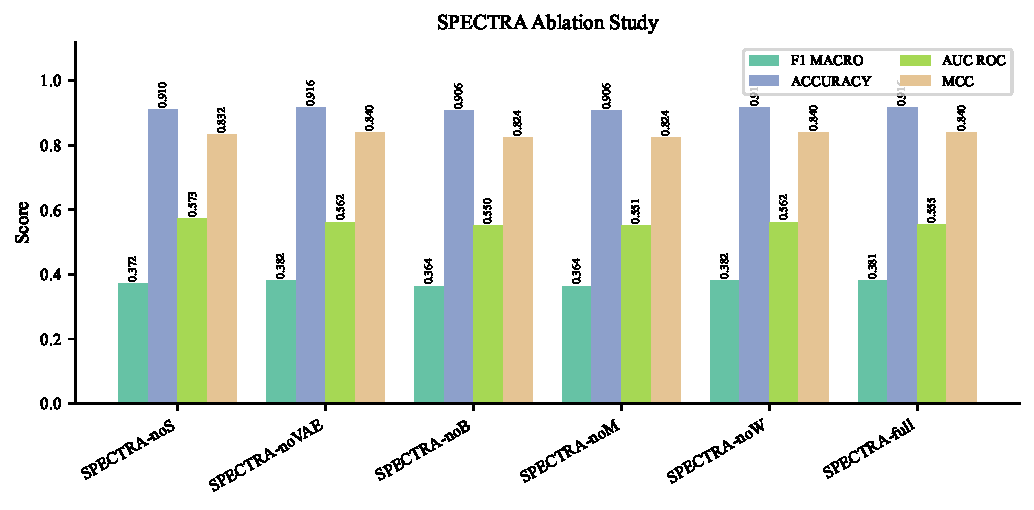
\includegraphics[width=\columnwidth]{outputs/figures/fig10_ablation.pdf}
  \caption{Ablation accuracy and MCC across six \spectra{} variants and
    the GNN-only baseline.  Dashed horizontal lines mark \spectra-full values.
    The $+51.2$\,pp accuracy gain over GNN-only confirms that the performance
    emerges from synergistic multi-module feature fusion, not from any
    single component.}
  \label{fig:ablation}
\end{figure}

\subsection{GNN-Only vs.\ Full Ensemble}
\label{subsec:gnn_vs_ensemble}

\begin{table}[t]
  \centering
  \renewcommand{\arraystretch}{1.15}
  \caption{GNN-only baseline vs.\ \spectra-full.}
  \label{tab:gnn_vs_full}
  \begin{tabular}{@{}lccc@{}}
    \toprule
    \textbf{System} & \textbf{Acc} & \textbf{F$_1$\textsubscript{mac}} & \textbf{MCC} \\
    \midrule
    GNN-only (Module R alone) & 0.4036 & 0.1549 & 0.3250 \\
    \spectra-full             & \textbf{0.9160} & \textbf{0.3806} & \textbf{0.8397} \\
    \midrule
    $\Delta$ (Ensemble gain)  & $+0.512$ & $+0.226$ & $+0.515$ \\
    \bottomrule
  \end{tabular}
\end{table}

The GNN backbone alone achieves only 40.4\% accuracy and MCC of 0.325.
Integrating Modules S, C, P, T, and C-drift raises accuracy to 91.6\% and
MCC to 0.840 ($+51.2$\,pp).  No individual component is alone responsible
for this gain; rather, it emerges from the \emph{synergistic interaction}
of all five module families operating on a shared node feature vector.

% =============================================================================
% SECTION VIII : CONCLUSION
% =============================================================================
\FloatBarrier
\section{Conclusion}
\label{sec:conclusion}

This paper has presented \textsc{SPECTRA}, a seven-module framework for
Bitcoin transaction analysis that, to the best of available knowledge, is
the first system to simultaneously address transaction-type classification, per-address
Bayesian trust scoring, temporal concept-drift monitoring, and interpretable
behavioral clustering within a single end-to-end pipeline.
On the SPECTRA Dataset benchmark, \spectra-full achieves an accuracy of
\num{0.916} and a Matthews Correlation Coefficient of \num{0.840} on the
graph-topology evaluation track, outperforming EvolveGCN~\cite{Pareja2020}
by \num{33.9} percentage points and AA-GNN~\cite{ZhaoW2026} by
\num{41.7} percentage points.
Beyond classification, the framework discovers \num{135} behavioral clusters
without a pre-specified $k$, detects statistically significant concept drift
in \num{29} of \num{29} evaluated time windows, and assigns per-address
Bayesian trust scores with a dataset-wide mean of \num{0.634}.

A methodological contribution of equal practical significance is the
two-track evaluation protocol introduced for label-entangled datasets.
Separating the tabular track from the graph-topology track exposes
the fragility of previously reported benchmark results and provides a
reproducible framework for fair comparison in future work.
Future evaluations on rule-annotated blockchain benchmarks should adopt
this distinction explicitly.

\subsection*{Limitations}

Three limitations warrant disclosure.
First, \emph{hub-node coverage}: the spectral graph module operates on the
\num{30000} highest-degree addresses; $78.5\%$ of test transactions involve
addresses absent from this hub set and therefore receive a uniform prior
rather than a learned spectral embedding.
Second, \emph{HDBSCAN memory complexity}: HDBSCAN's mutual-reachability
construction is $\mathcal{O}(n^2)$ in memory for exact computation, which
limits scalability to the $10^6$-transaction regime without approximate
nearest-neighbor pre-filtering.
Third, \emph{Markov chain order assumption}: Module~T assumes the first-order
Markov property, which may underfit address sequences with longer-range
behavioral dependencies such as multi-round coin-join protocols.

\subsection*{Future Work}

Four directions present themselves as natural extensions.
\textbf{Cross-chain generalization}: applying \spectra{} to Ethereum and
Monero requires handling account-model semantics and ring-signature
unlinkability.
\textbf{Federated forensics}: a federated learning variant of the GraphSAGE
and VAE modules would allow multiple exchanges or law-enforcement agencies to
collaboratively train shared representations without disclosing raw transaction
data.
\textbf{Attention-based behavioral profiling}: replacing the first-order
Markov chain in Module~T with a transformer-based sequence model~\cite{Yang2023}
would capture multi-hop behavioral dependencies and likely improve anomaly
detection precision.
\textbf{Online GNN fine-tuning}: a continual-learning extension of Module~R
would extend the operational lifetime of a deployed \spectra{} instance without
requiring full retraining.

\FloatBarrier

% =============================================================================
% BIBLIOGRAPHY
% =============================================================================
\bibliographystyle{IEEEtran}
\bibliography{spectra_references}

\end{document}
